% Preamble
\documentclass[a4paper,12pt]{article}

\usepackage[osf]{mathpazo} % palatino
\usepackage{ms}            % load the template
%\usepackage[round]{natbib} % author-year citations
\usepackage[superscript,biblabel]{cite} % for superscript citations
\usepackage{graphicx}
\usepackage{parskip} 
\usepackage{caption}
\usepackage{subcaption}
\usepackage{textcomp} % for parts per mille symbol     
\pagenumbering{arabic}    
\linespread{1.66}

% Title page information
\title{Reconstructing the last known movements of one of Nature's giants}
% 90 characters max

\author{
  Natalie Cooper$^{1*}$ Andrew L. Jackson$^{2}$, Katharyn S. Chadwick$^{3}$,\\ Ellen J. Coombs$^{1,4}$,
  Richard C. Sabin$^{1}$ and Clive N. Trueman$^{3}$ 
}
\date{}
\affiliation{\noindent{\footnotesize
  $^1$ Department of Life Sciences, Natural History Museum London, Cromwell Road, London, SW7 5BD, UK.\\ 
  $^2$ School of Natural Sciences, Trinity College Dublin, Dublin 2, Ireland.\\
  $^3$ National Oceanographic Centre, University of Southampton, Southampton, UK.\\
  $^4$ University College London, Gower Street, London, WC1E 6BT, UK.\\
}}

\vfill

%\runninghead{}
%\keywords{}
%}

% End of preamble

\begin{document}
\modulolinenumbers[1]   % Line numbering on every line

\mstitlepage

\parindent = 1.5em
\addtolength{\parskip}{.3em}
% Abstract 200 -300 words max
% \section{Abstract}
% general topic intro - 1 sentence
% intro to field - 2 sentences
% what we find/show - 1 sentence
% implications - 2-3 sentences. Results in context, how has the paper moved the field forward

\paragraph{Understanding animal movements is crucial for effective conservation, especially as species ranges shift due to climate change\cite{runge2014conserving,robinson2009travelling}. 
Animal tissues housed in museum collections provide biochemical records of behaviour that can be used to reconstruct individual-level movements over long time scales and under historic climatic and ecological conditions\cite{newsome2010using}. 
Here we combine stable isotope analyses of baleen with novel agent-based simulation models, to reconstruct movements over the last six years of the life of an iconic blue whale (\textit{Balaenoptera musculus}) that stranded off Ireland in 1891 and is now on display at the Natural History Museum, London (NHM). 
We identify two distinct phases in the whale's behaviour: repeated annual north-south migrations in sub-Arctic waters, and residency in subtropical waters. 
Subtropical residency is associated with isotopic signatures consistent with pregnancy and lactation in the year before the whale’s death. 
These results supply the first quantitative multi-yeat records of historical migrations in individual blue whales, and suggest that blue whale residency and movement patterns in the North Atlantic have remained similar for hundreds of years, despite changing human pressures in the region. 
Historic tissue collections can provide unique insight into individual-level movement behaviours associated with changing climatic, ecological conditions and human-induced pressures, and reveal aspects of life history. 
Combining biochemical tracers with simulation modelling unlocks the information recorded in these irreplaceable archives.}

%\section{Main text}
% 1500 words max (excludes refs title, authors, abstract, acknowledgements)
\newpage

Migratory species pose a particular challenge for conservation practitioners, because their effective conservation relies on protection at many, often very distant, sites\cite{runge2014conserving}. 
Such species are also likely to be particularly vulnerable to climate change, as changes may impact various parts of their life cycle\cite{robinson2009travelling}. 
Dealing with these issues is difficult due to the relative scarcity of information on individual-level movements over multiple years, for both historical and present-day populations, particularly for wide-ranging marine species\cite{ryan2013stable,hall2005stable,bailey2009behavioural}. 
 
The blue whale (\textit{Balaenoptera musculus}), the largest animal to have ever lived on Earth, is one such migratory marine species. 
Despite blue whale hunting being banned for over 50 years, blue whales are still listed as Endangered by the IUCN Red List\cite{reilly2008balaenoptera}.
Conservation efforts are hampered by the scarcity of detailed data on blue whale distribution, behaviour and ecology, for both historical and present-day populations. 
Current methods for tracking large whales include satellite tracking, radio tagging, aerial photography, passive acoustic monitoring, and sightings records\cite{borger15,mcdonald2006biogeographic,bailey2009behavioural,mate2007evolution}). 
These methods are adding vital behavioural data to our understanding of whale movements, however, they are expensive, often limited to short-term studies on few individuals\cite{bailey2009behavioural,best2015tag,mate2007evolution}, and may influence whale behaviour\cite{walker2012review}. 
An alternative technique is to investigate oscillations in stable isotopes values of whale tissues housed in museum collections\cite{ryan2013stable}.
This is a non-invasive method that provides individual-level movement information at high temporal resolution over multiple years. 
Here we apply this method to baleen from the Natural History Museum's blue whale.
 
Baleen is formed of plates of keratin and is used by mysticete whales to filter feed. 
It is ideal for stable isotope studies because keratin grows continuously through an individual's life, and once laid down it is metabolically inert\cite{best1996stable}. 
We sampled keratin from the blue whale's baleen plate at 1cm intervals and used continuous-flow isotope ratio mass spectrometry to extract $\delta^{13}$C and $\delta^{15}$N isotope concentrations. 
Given the date of stranding (25th March 1891), and estimated baleen growth rates of 13.5cm $y^{-1}$ (see Supplemental Methods), we reconstructed a timeline for $\delta^{13}$C and $\delta^{15}$N fluctuations in the baleen over the last six years of whale's life (autumn 1885 - spring 1891). The $\delta^{13}$C and $\delta^{15}$N profiles show two distinct phases in the whale's behaviour. 
In behavioural phase one (month 1885 to May 1889), we find strong cyclical fluctuations in both $\delta^{13}$C and $\delta^{15}$N values of an approximately yearly periodicity (Fig. 1). $\delta^{13}$C and $\delta^{15}$N exhibit strong negative covariance. 
In behavioural phase two (June 1889 to March 1891) we see a sharp uptick in $\delta^{13}$C, followed by high and relatively constant $\delta^{13}$C values. ,
This is associated with an overall reduction in $\delta^{15}$N values and a weakening of the periodic $\delta^{15}$N fluctuations seen in behavioural phase one. There is also no covariance between $\delta^{13}$C and $\delta^{15}$N (Fig. 1). 

%  \begin{figure}[!htbp]
%    \centering
%      \includegraphics[width=12cm]{XXX.pdf}
%      \caption{}
%      \label{}
%  \end{figure}

% 2 panel figure of the two traces - real and simulated

\begin{figure}
  \centering
    \begin{subfigure}{0.8\textwidth}
      \centering
      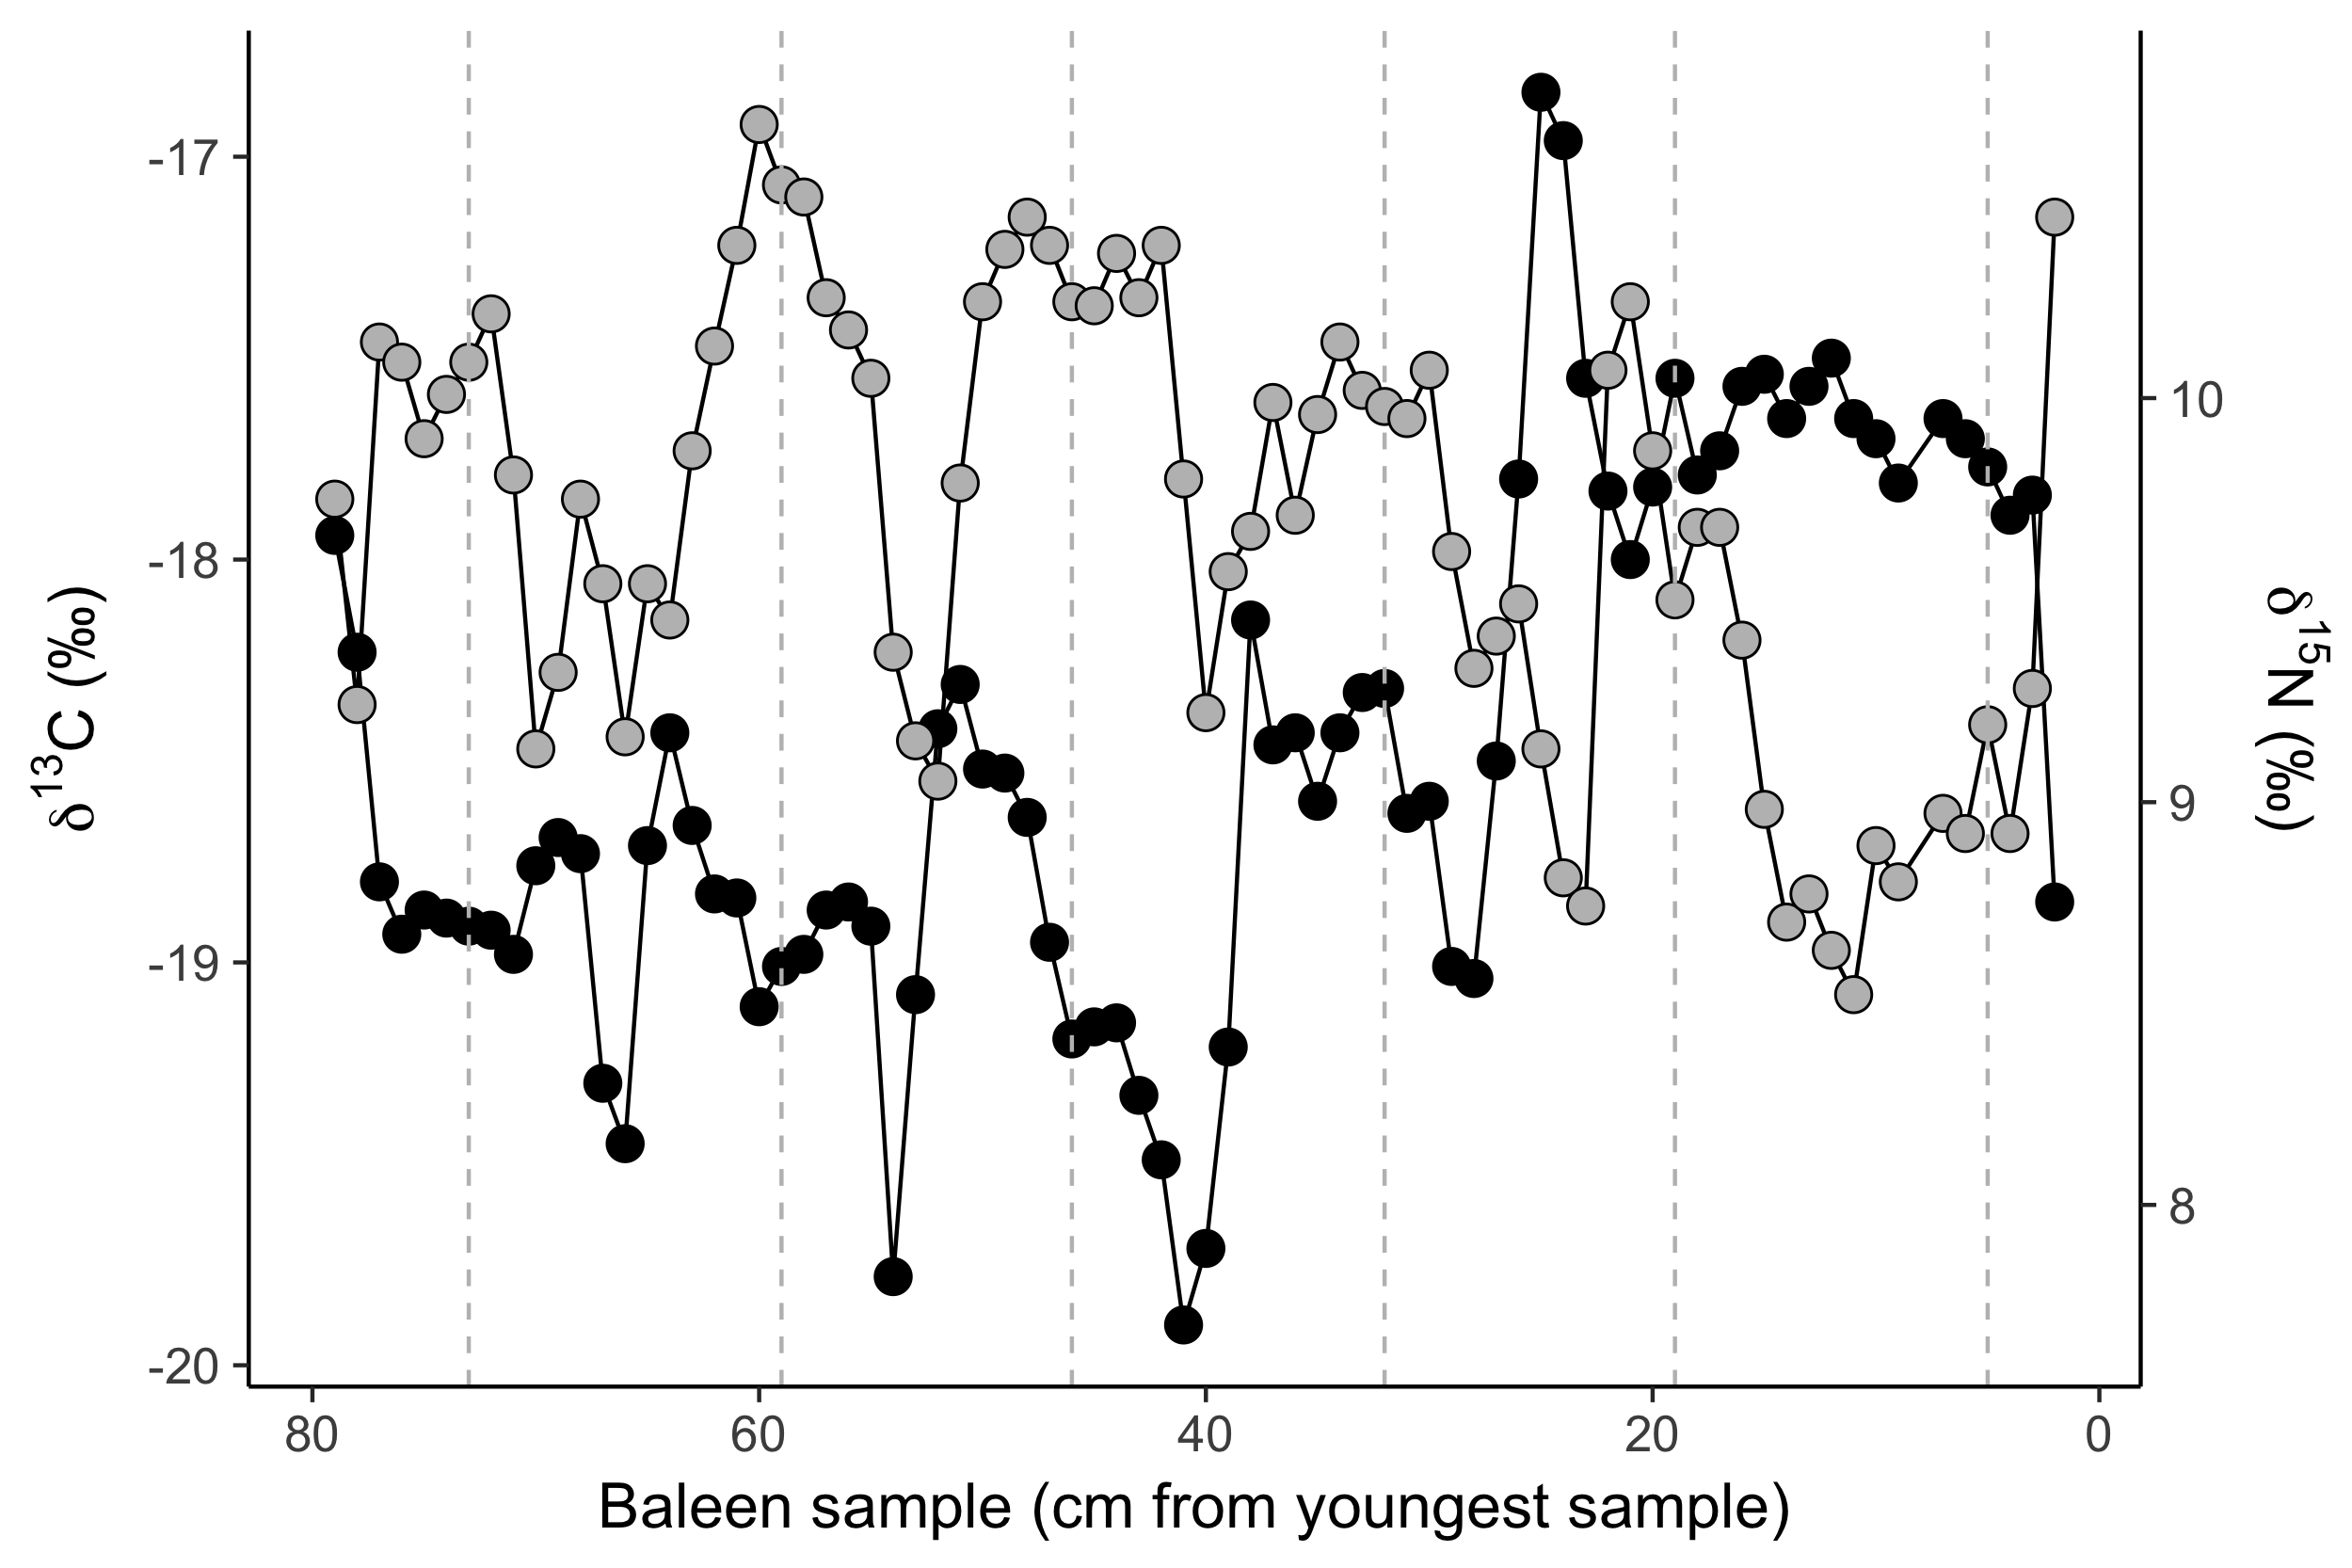
\includegraphics[width = \linewidth]{figures/Figure-1a-raw-dC-dN-data.png}
      \label{fig1a}
    \end{subfigure}

    \begin{subfigure}{0.8\textwidth}
      \centering
      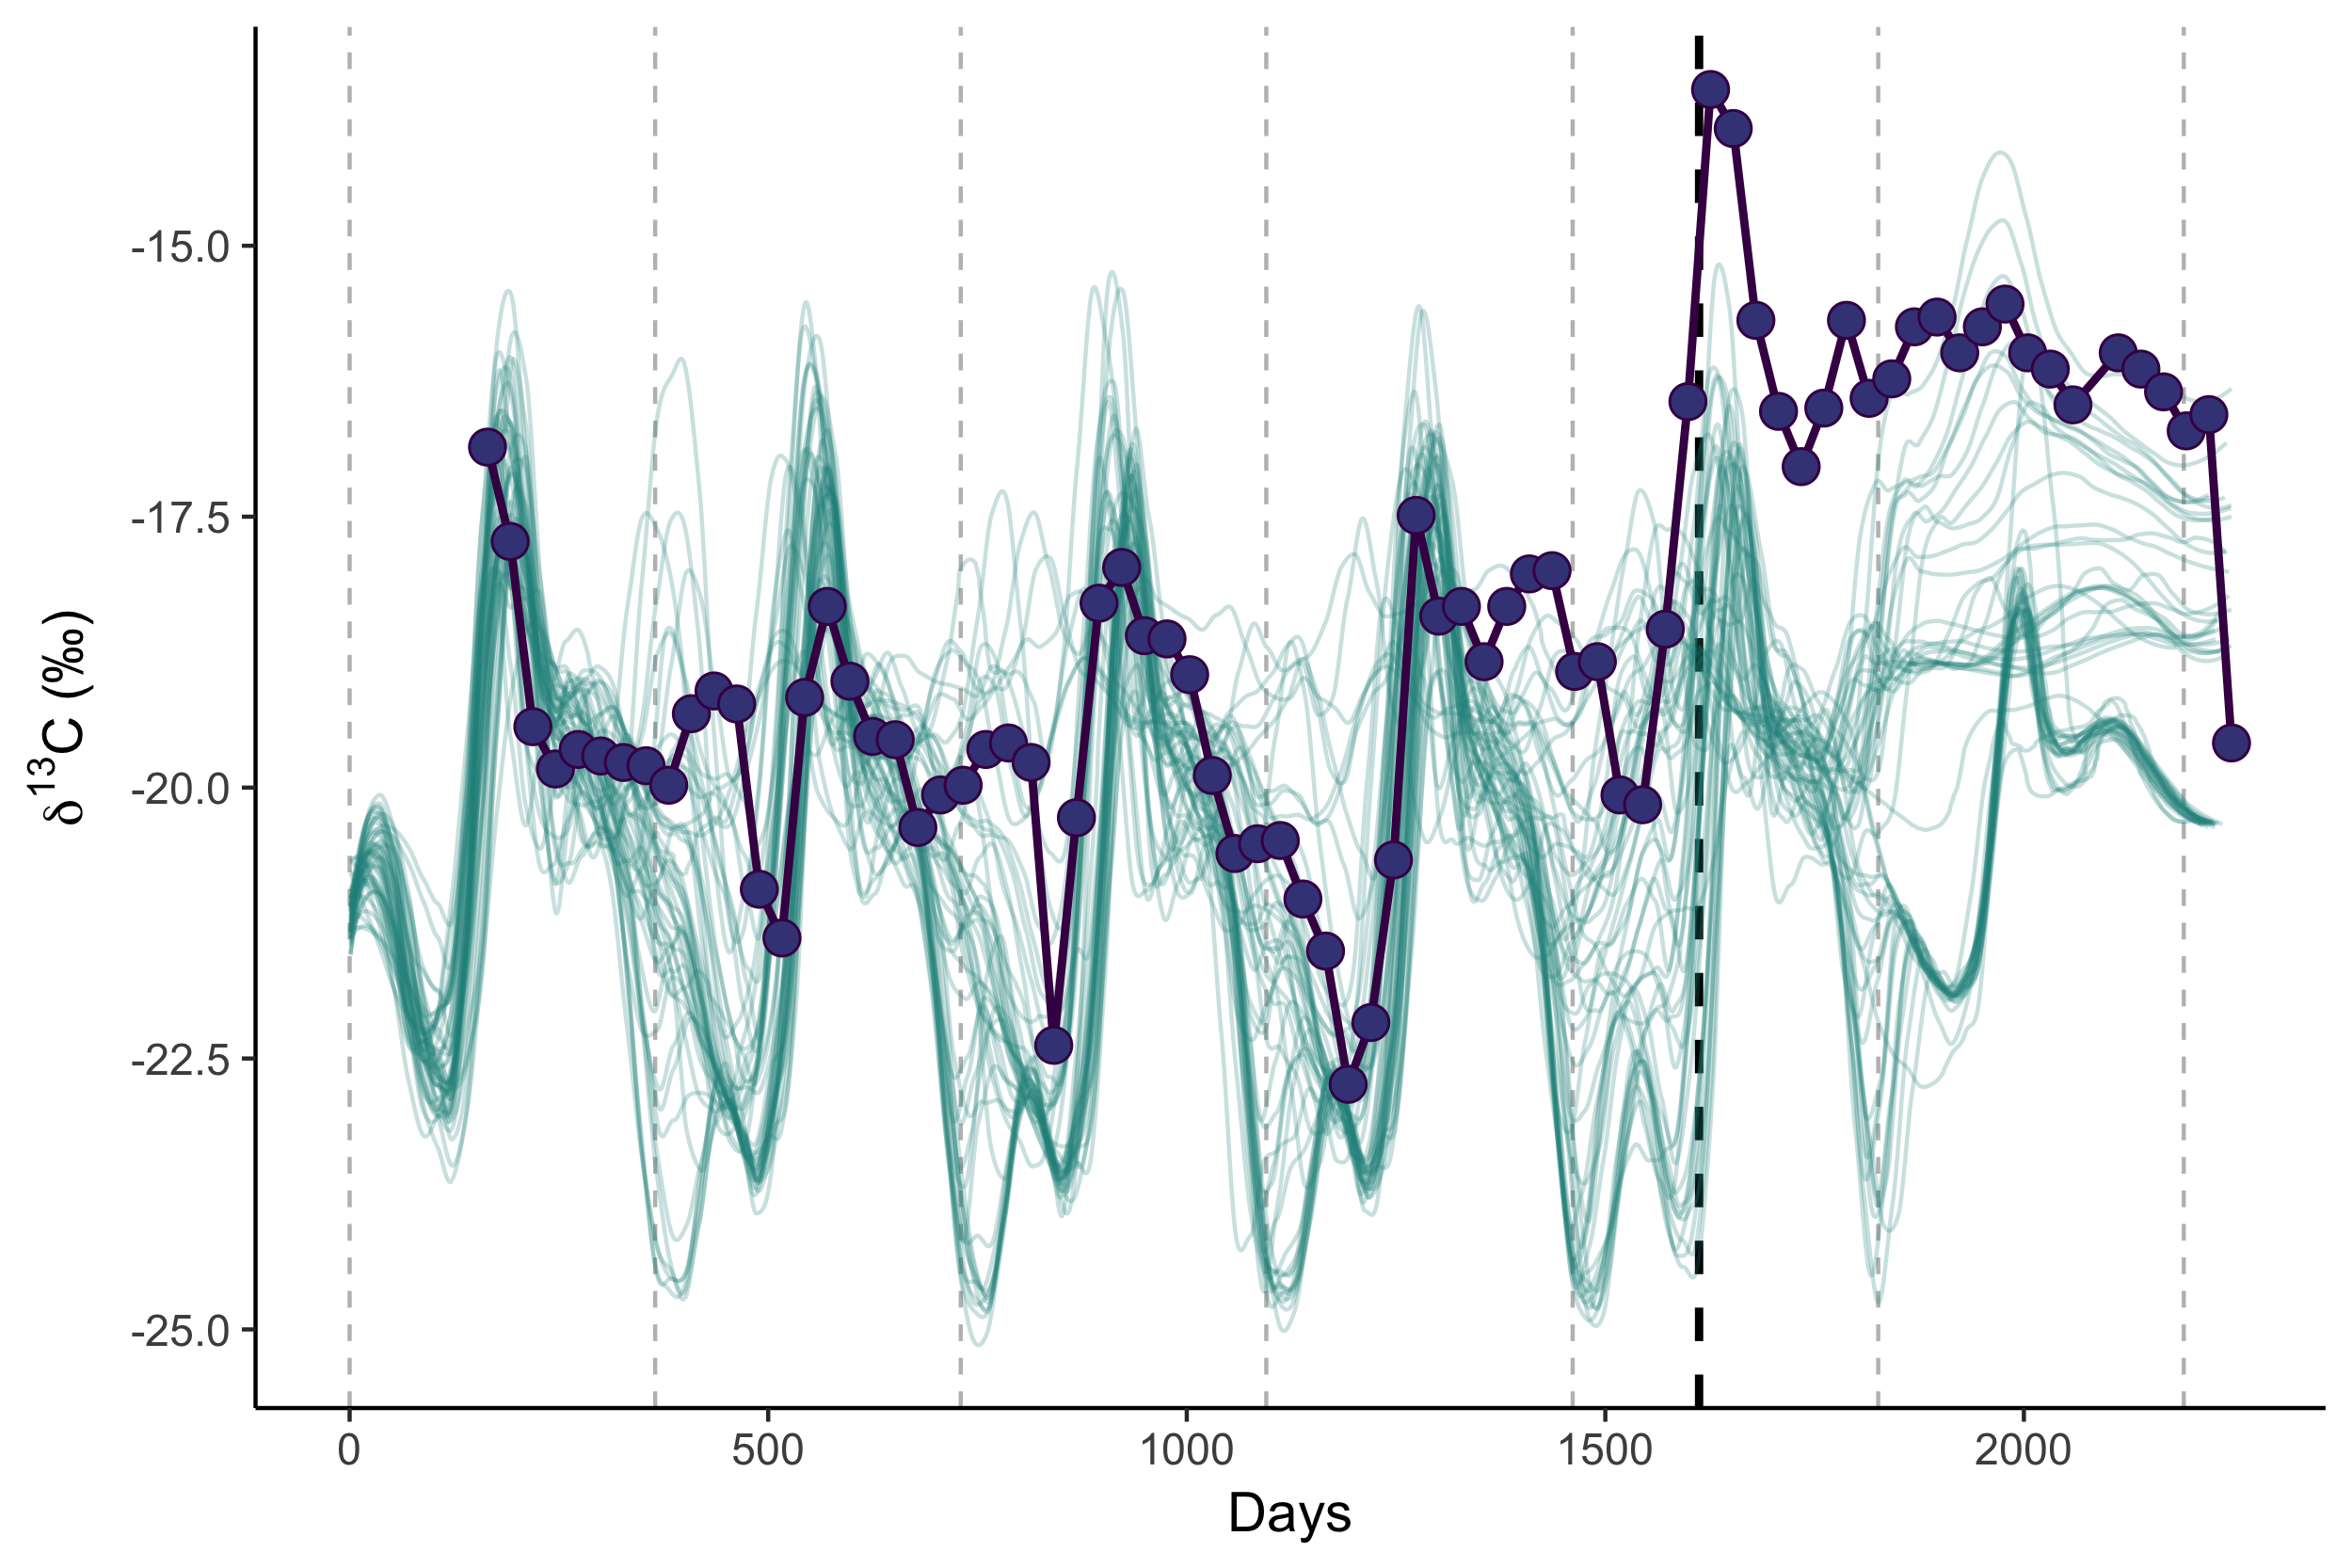
\includegraphics[width = \linewidth]{figures/Figure-1c-migratory-model-d13C.png}
      \label{fig1b}
    \end{subfigure} 
  \caption{Two panel figure with two traces}
\end{figure}

% two panel with the simulations and map
\begin{figure}
  \centering
    \begin{subfigure}[b]{0.45\textwidth}
      \centering
      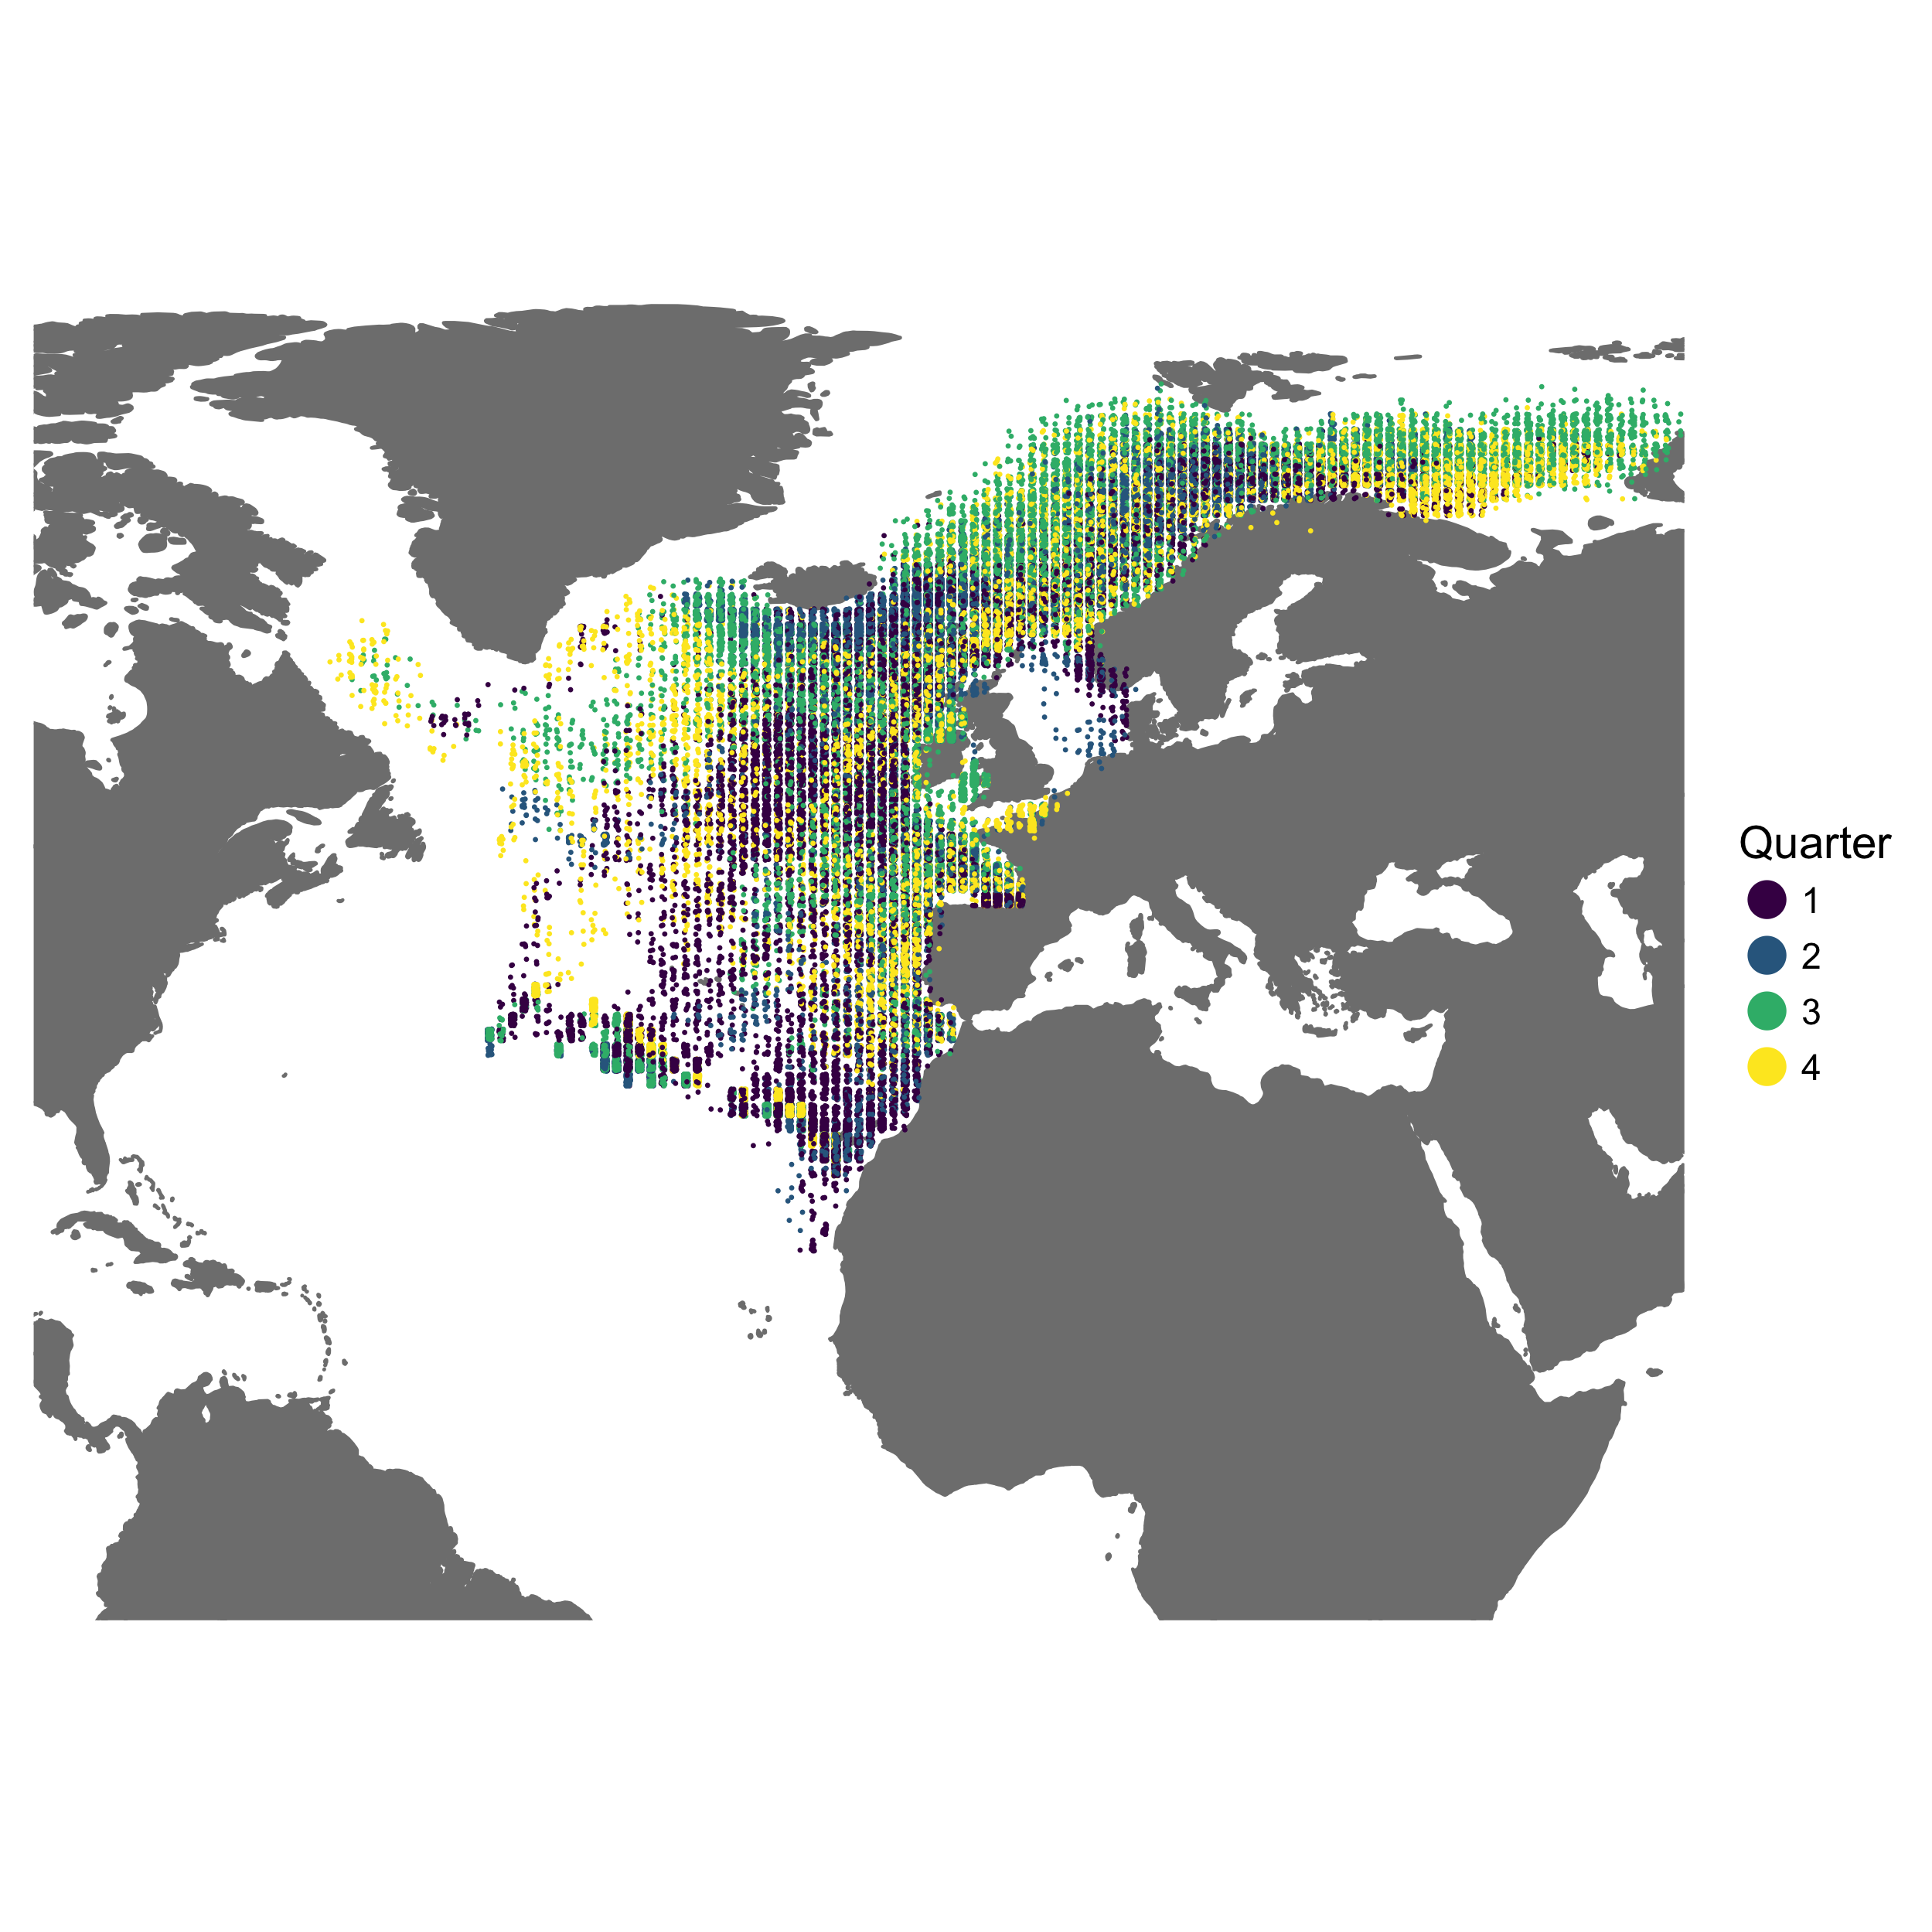
\includegraphics[width = \linewidth]{figures/Figure-1b-migratory-model-full-map.png}
      \label{fig2a}
    \end{subfigure}
    \begin{subfigure}[b]{0.45\textwidth}
      \centering
      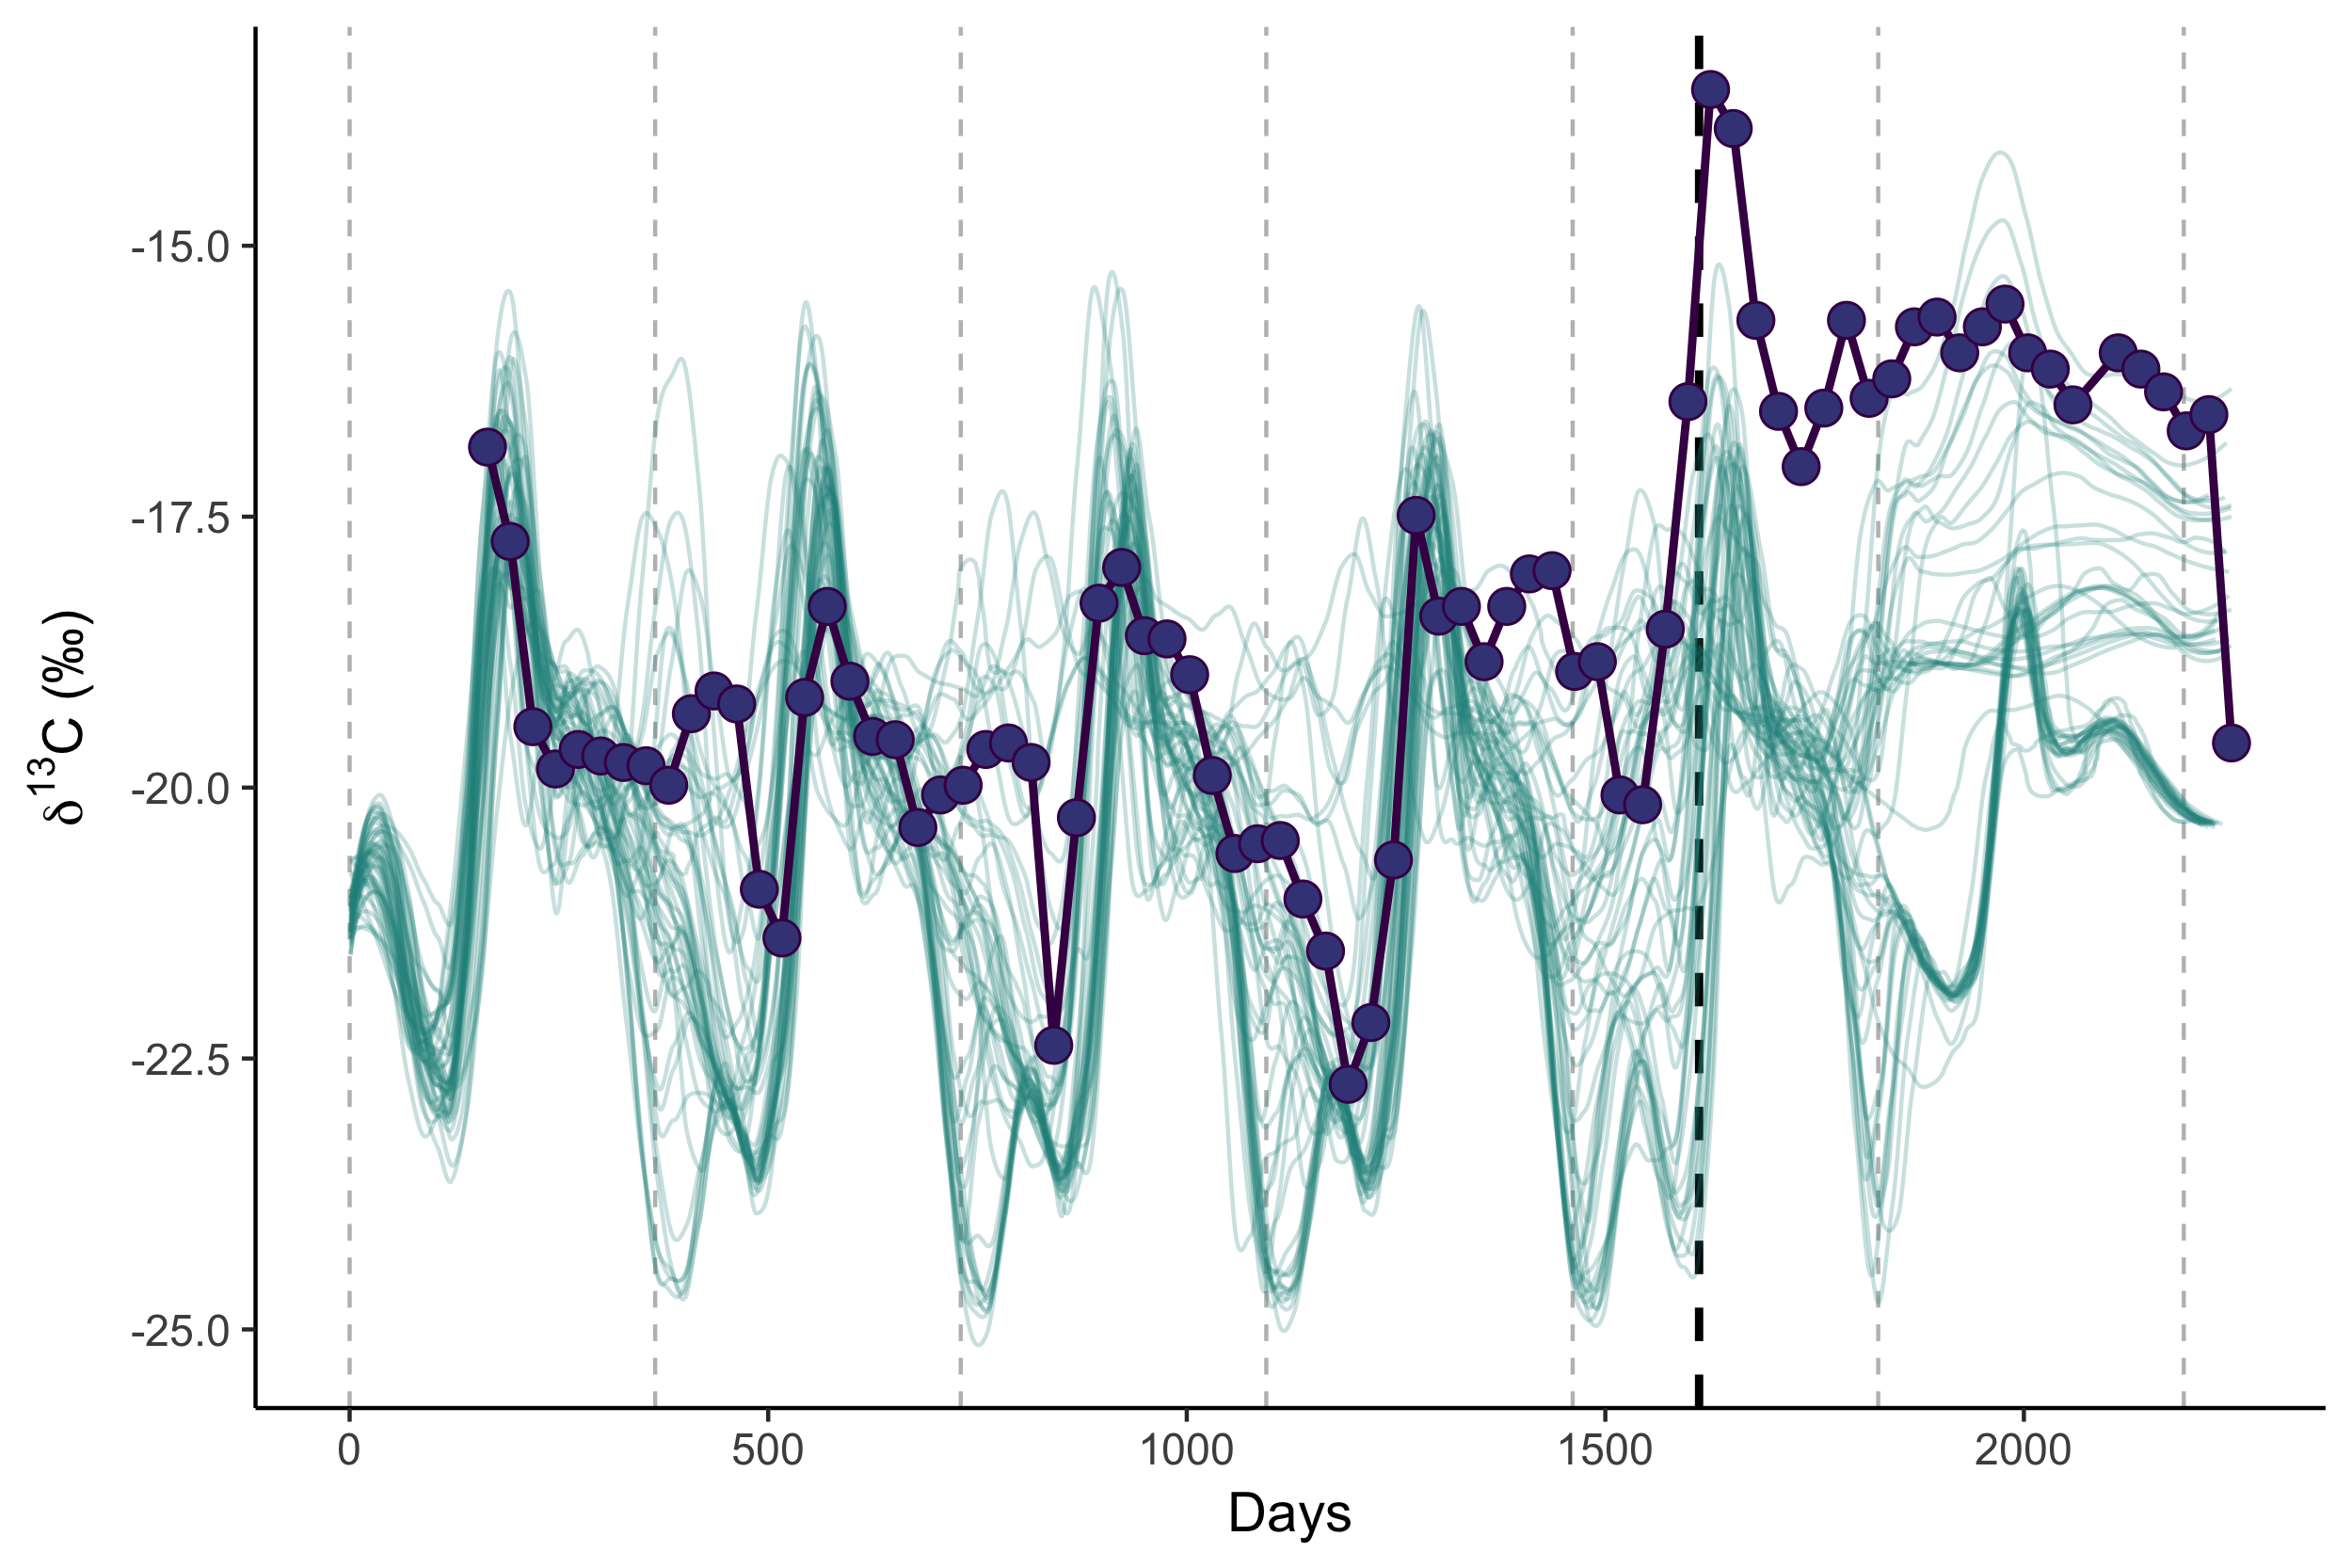
\includegraphics[width = \linewidth]{figures/Figure-1c-migratory-model-d13C.png}
      \label{fig2b}
    \end{subfigure} 
  \caption{Two panel figure with trace and map}
\end{figure}

% two panel with the simulations and map
\begin{figure}
  \centering
    \begin{subfigure}[b]{0.45\textwidth}
      \centering
      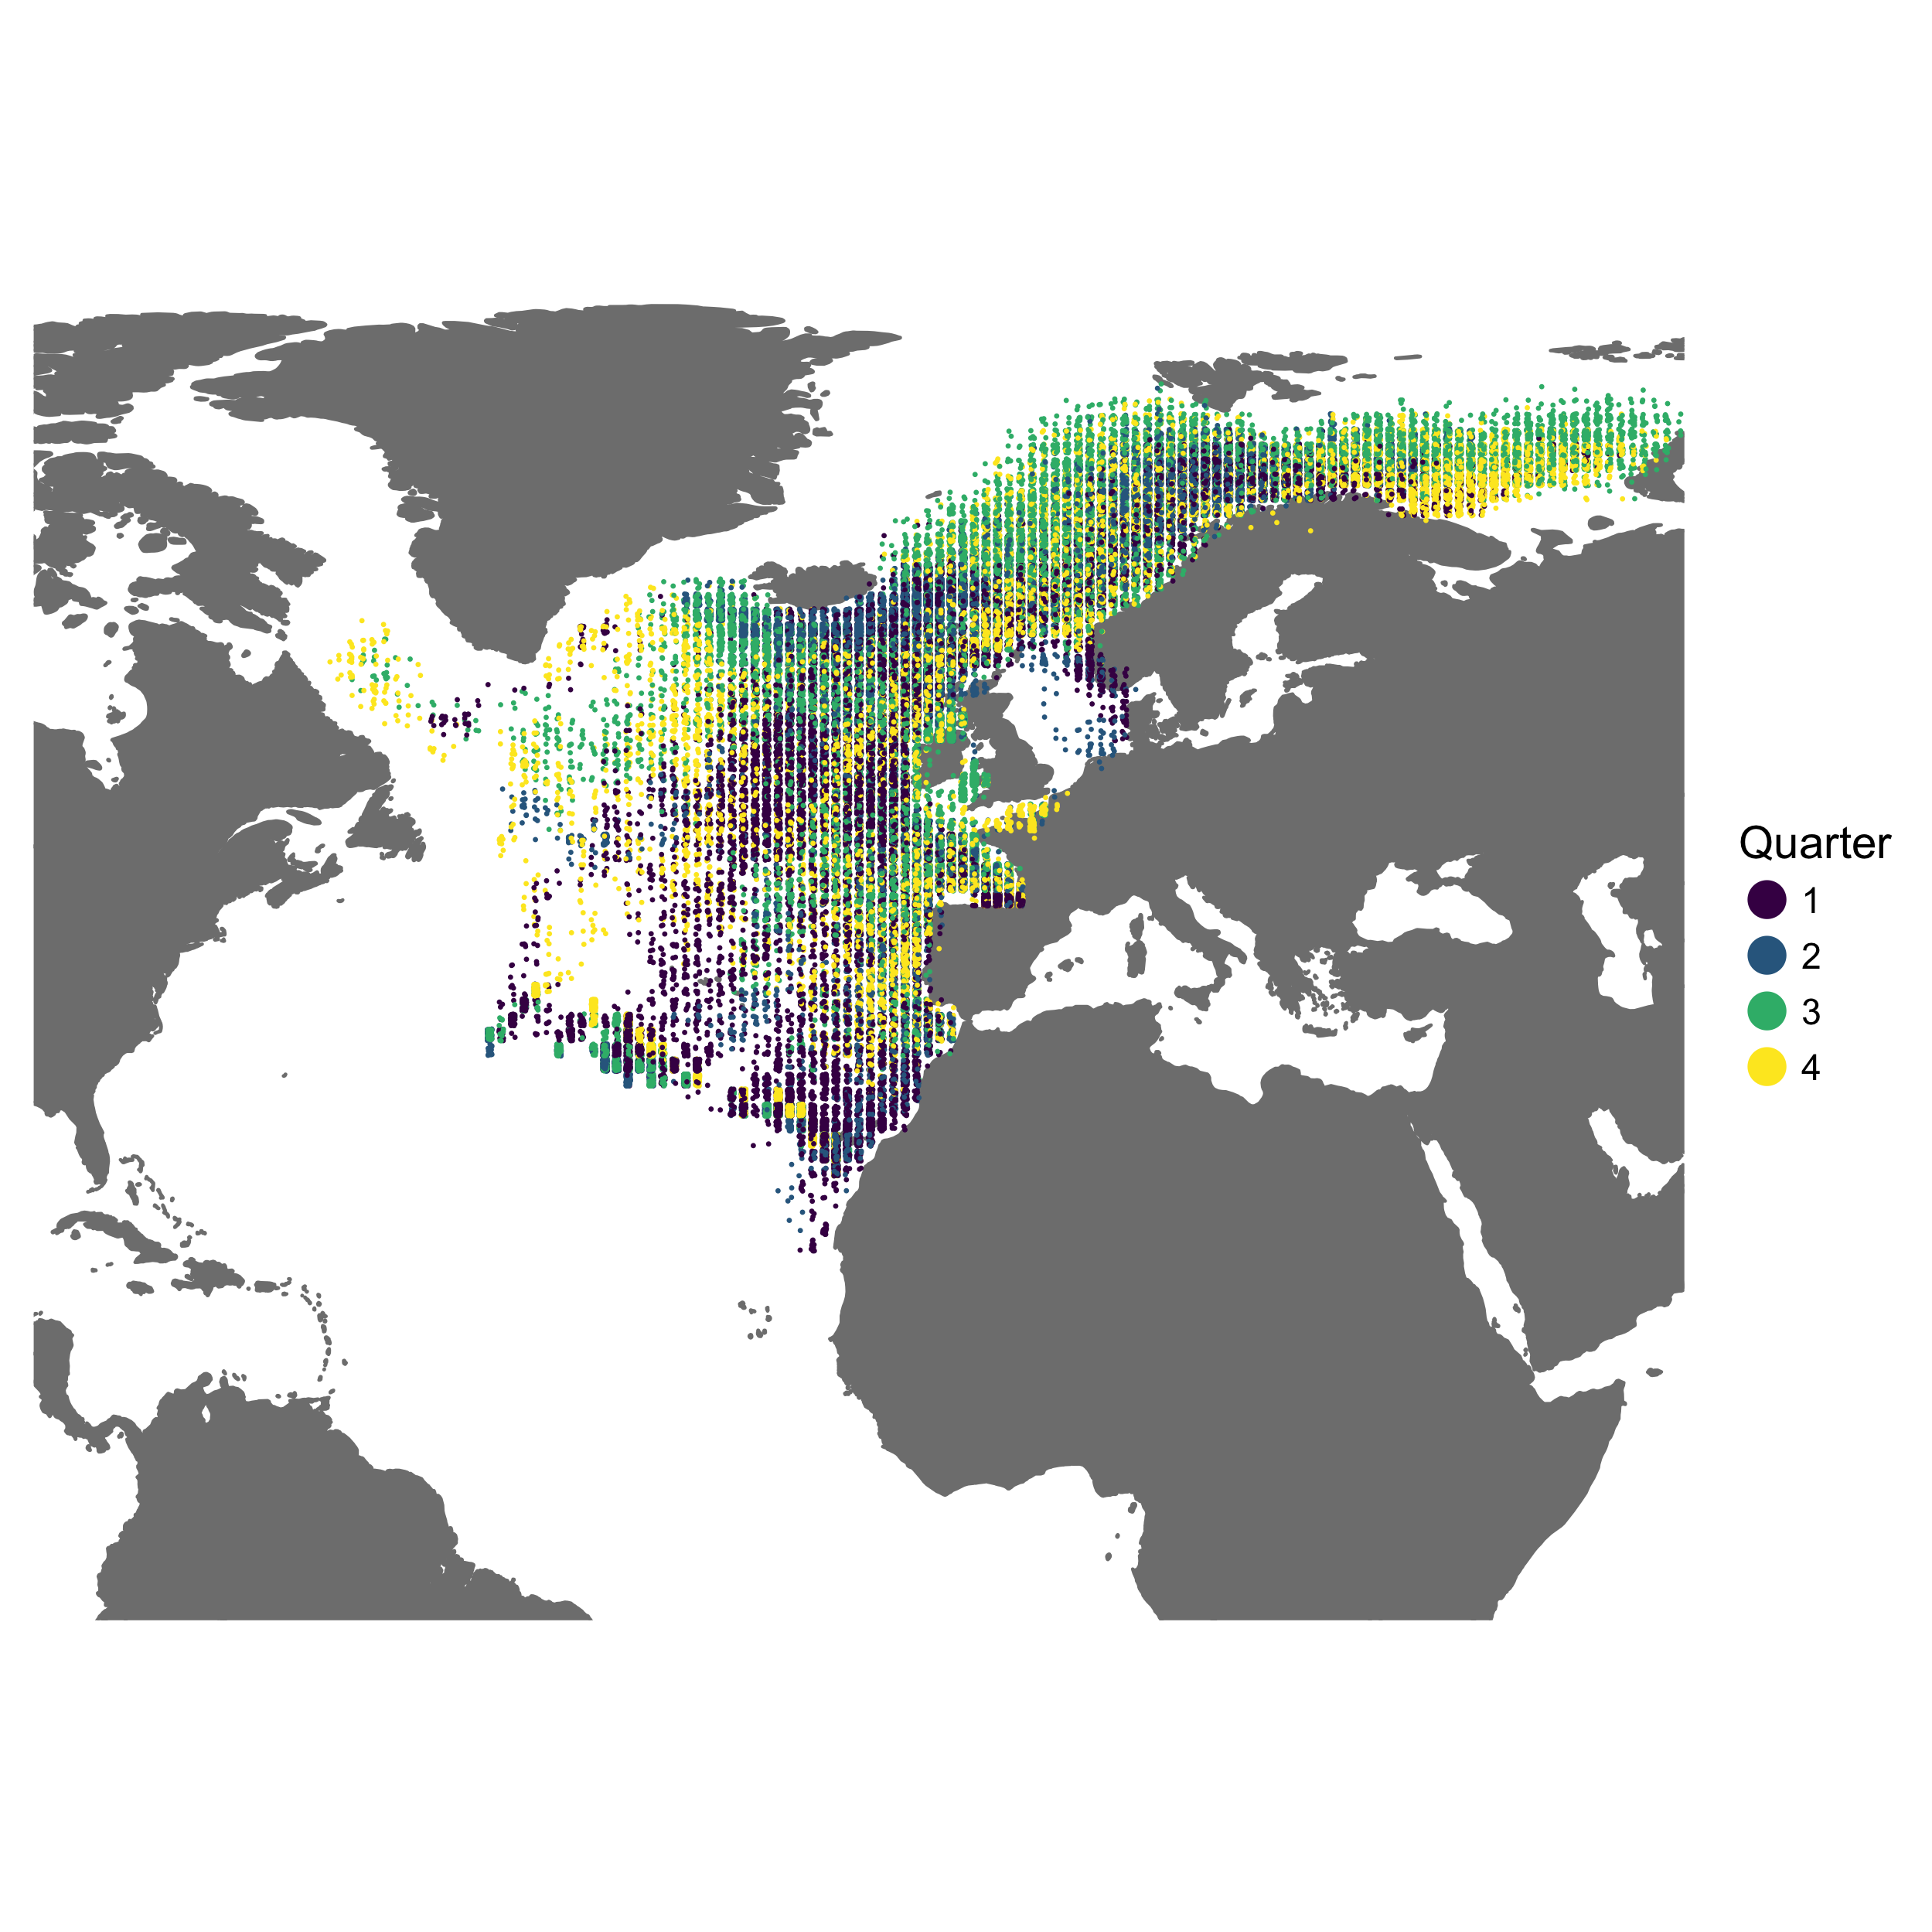
\includegraphics[width = \linewidth]{figures/Figure-1b-migratory-model-full-map.png}
      \label{figa}
    \end{subfigure}

    \begin{subfigure}[b]{0.45\textwidth}
      \centering
      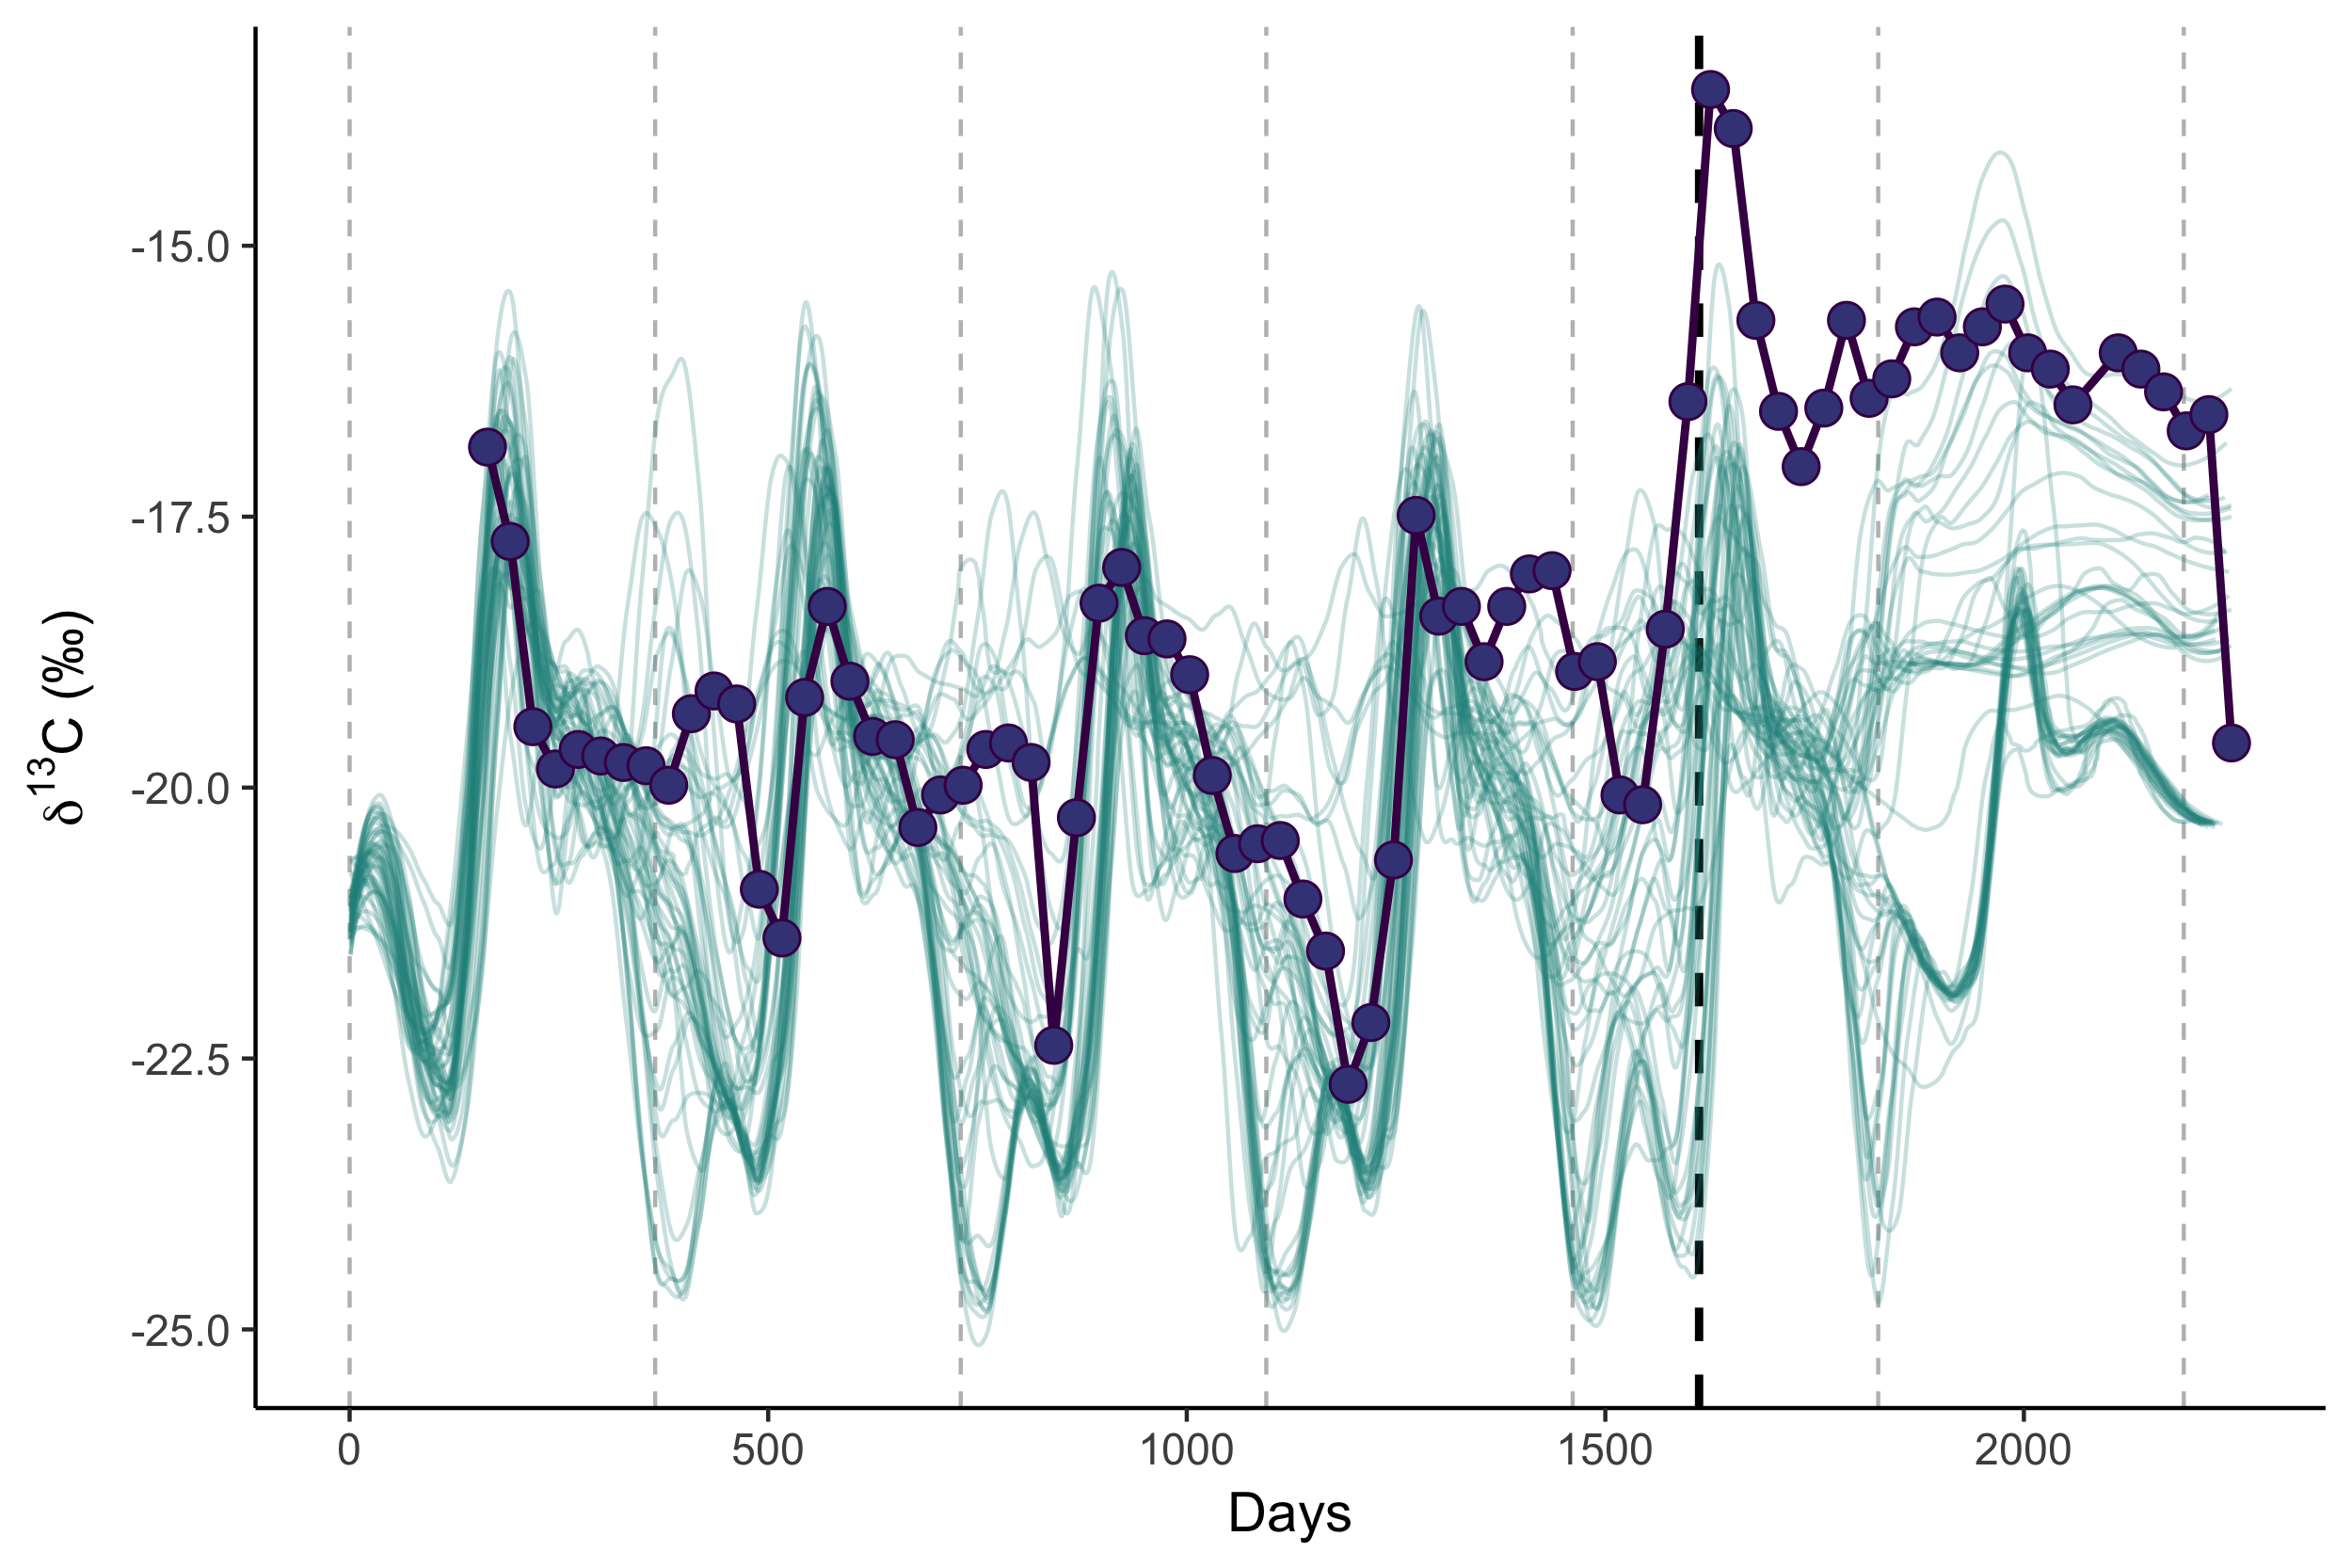
\includegraphics[width = \linewidth]{figures/Figure-1c-migratory-model-d13C.png}
      \label{figb}
    \end{subfigure} 
  \caption{Two panel figure with trace and map}
\end{figure}

% two panel with the simulations and map
\begin{figure}
  \centering
    \begin{subfigure}[b]{0.45\textwidth}
      \centering
      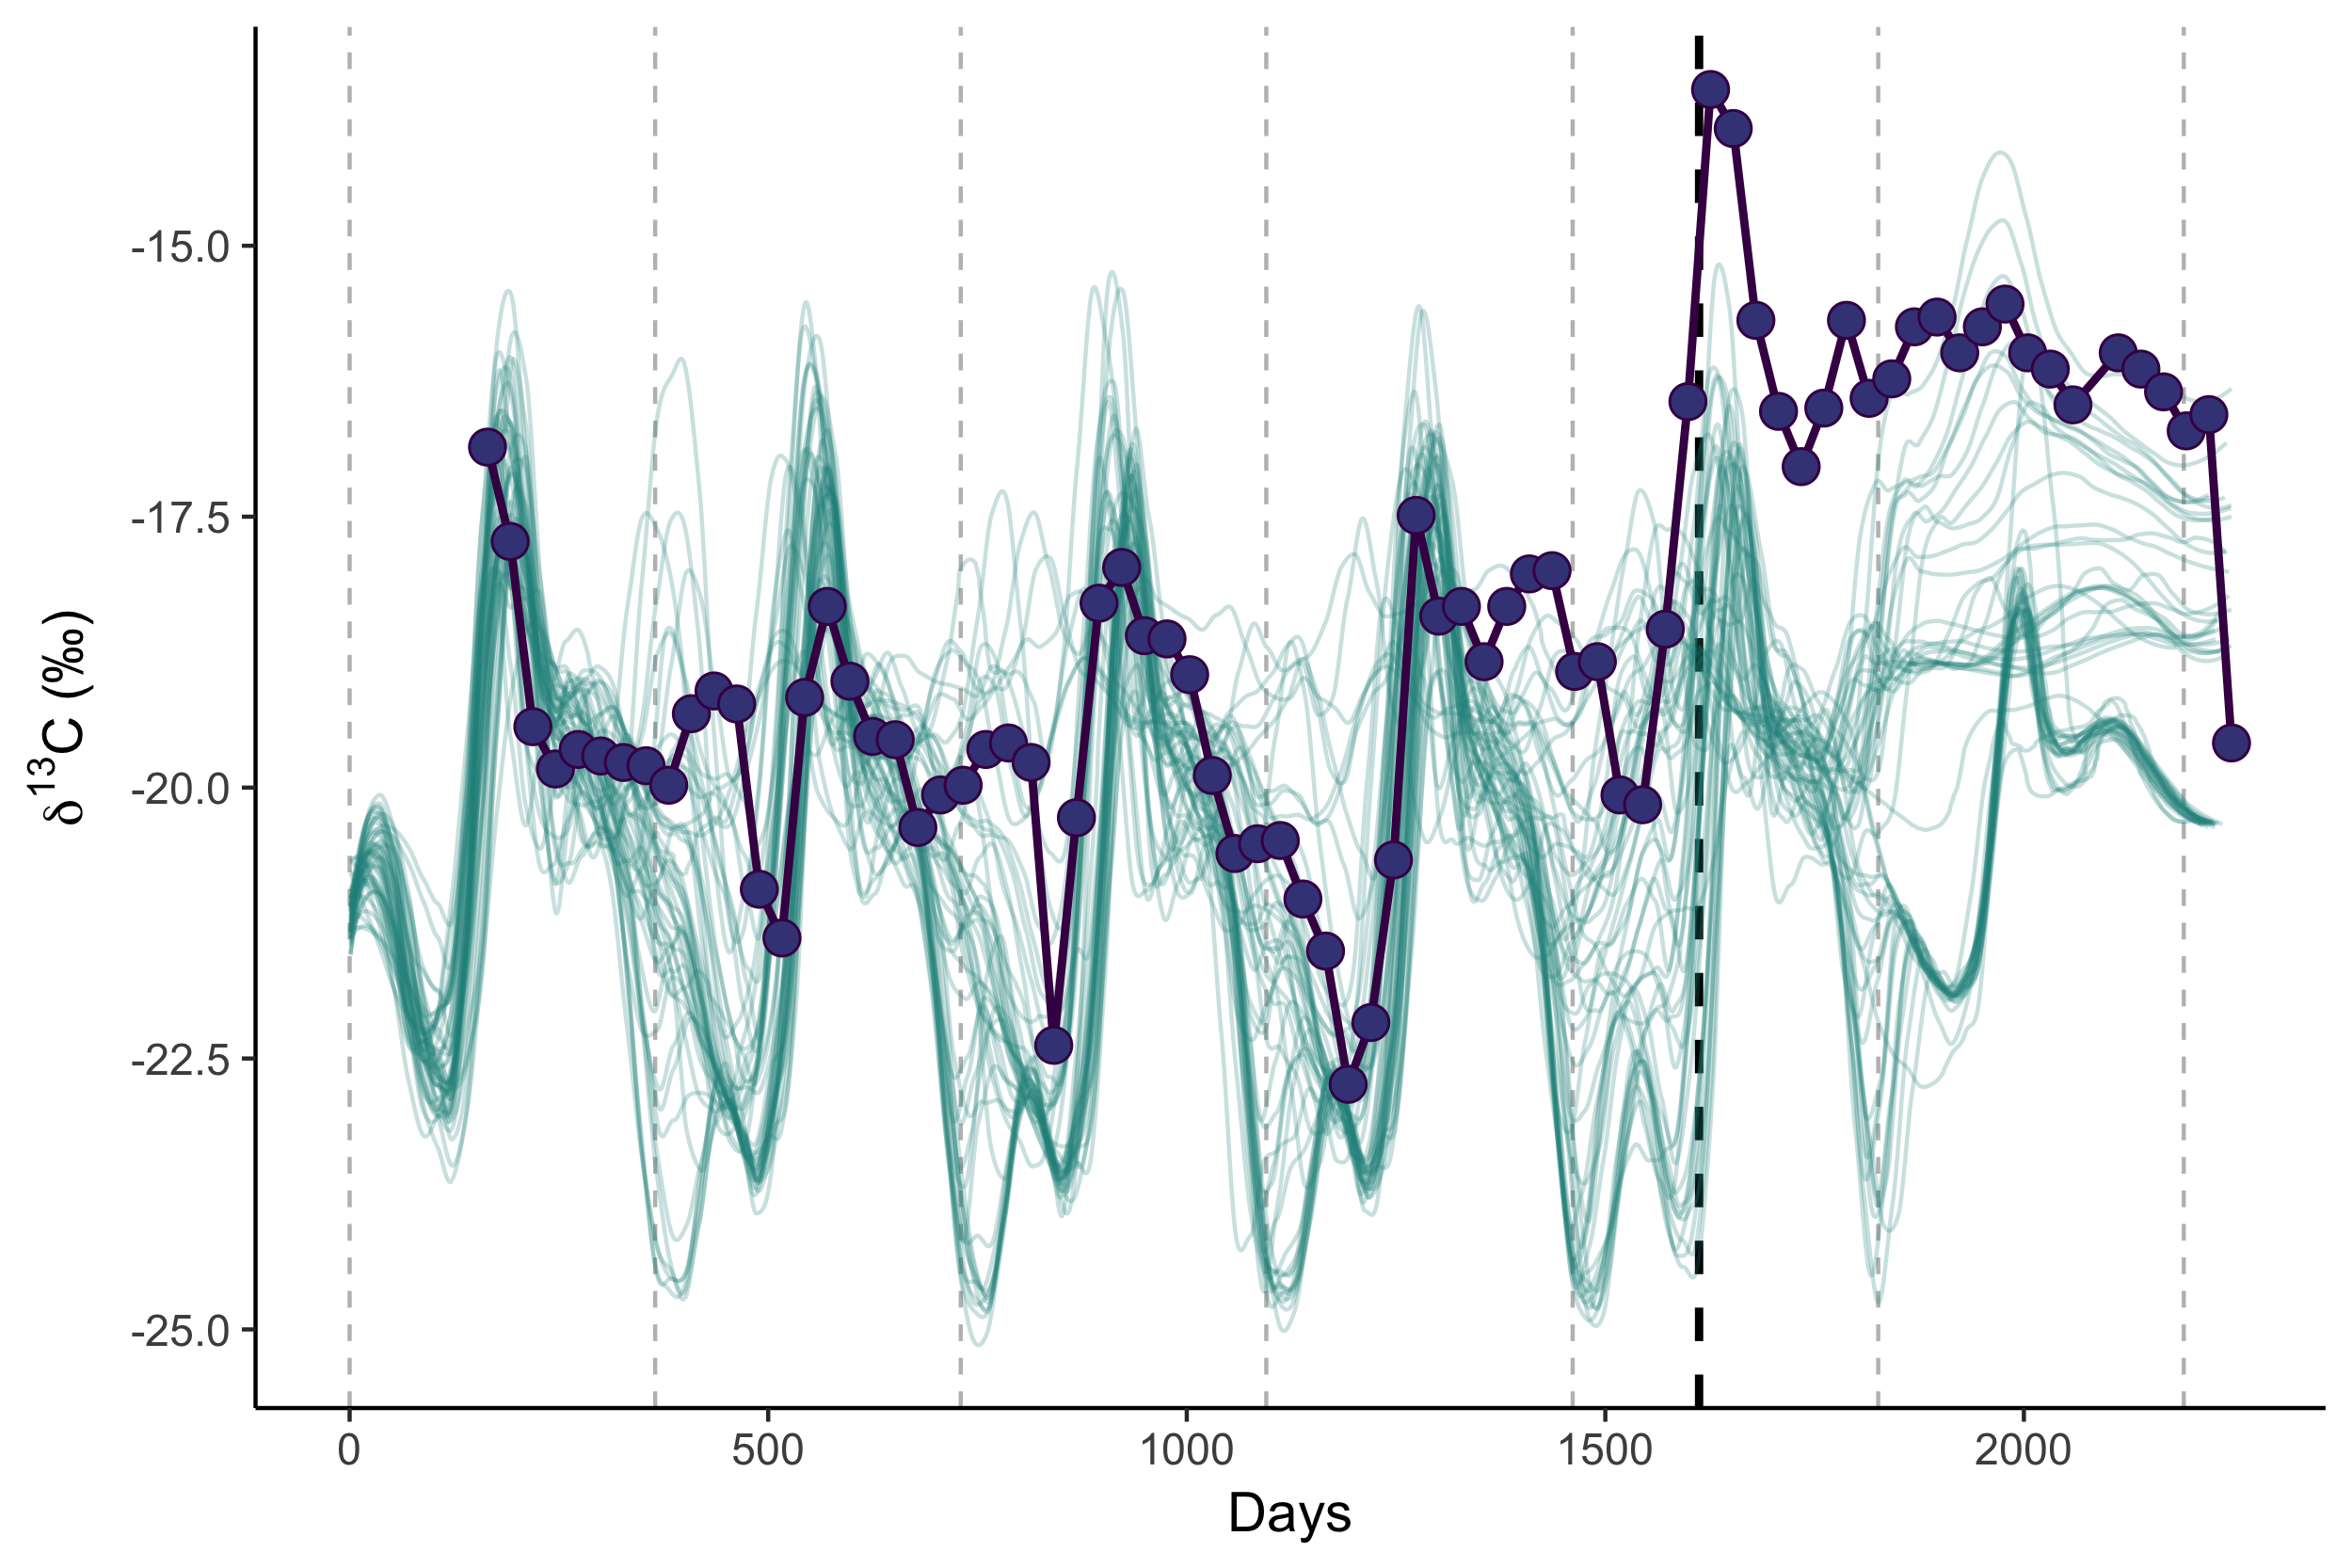
\includegraphics[width = \linewidth]{figures/Figure-1c-migratory-model-d13C.png}
      \label{fig3a}
    \end{subfigure}
    \begin{subfigure}[b]{0.45\textwidth}
      \centering
      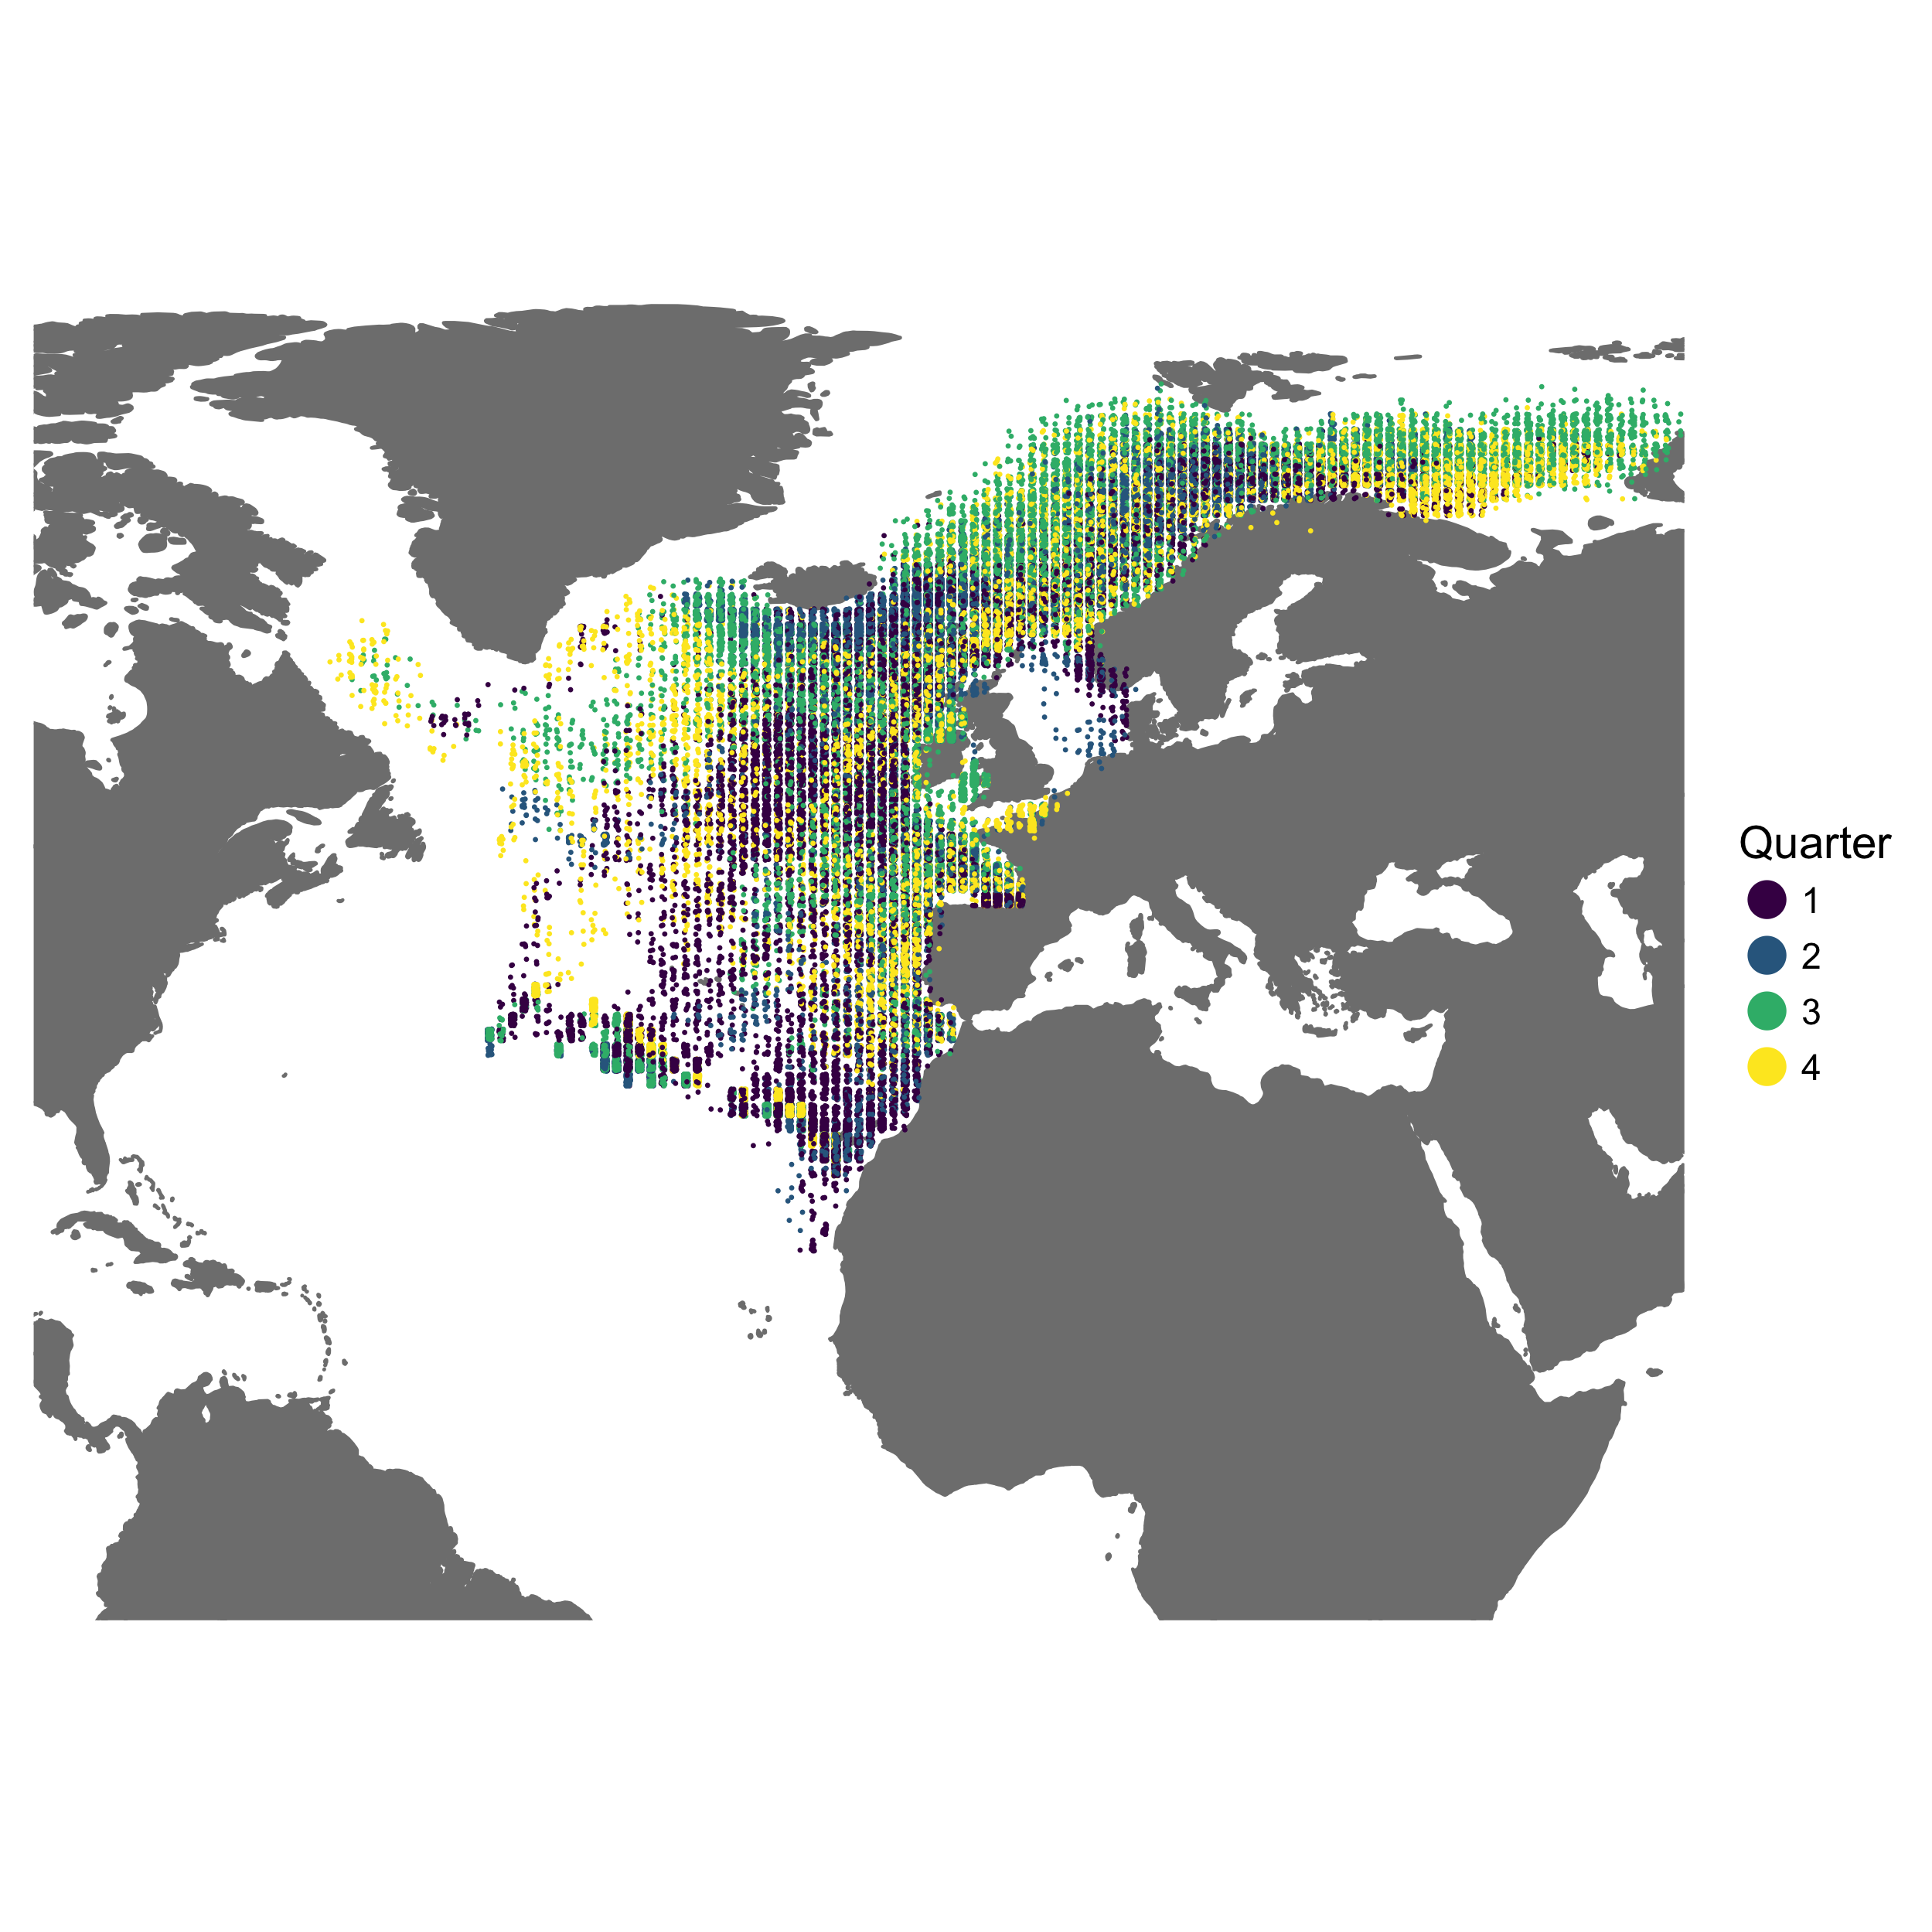
\includegraphics[width = \linewidth]{figures/Figure-1b-migratory-model-full-map.png}
      \label{fig3b}
    \end{subfigure} 
  \caption{Two panel figure with trace and map}
\end{figure}

% one panel of the real trace
\begin{figure}
  \centering
  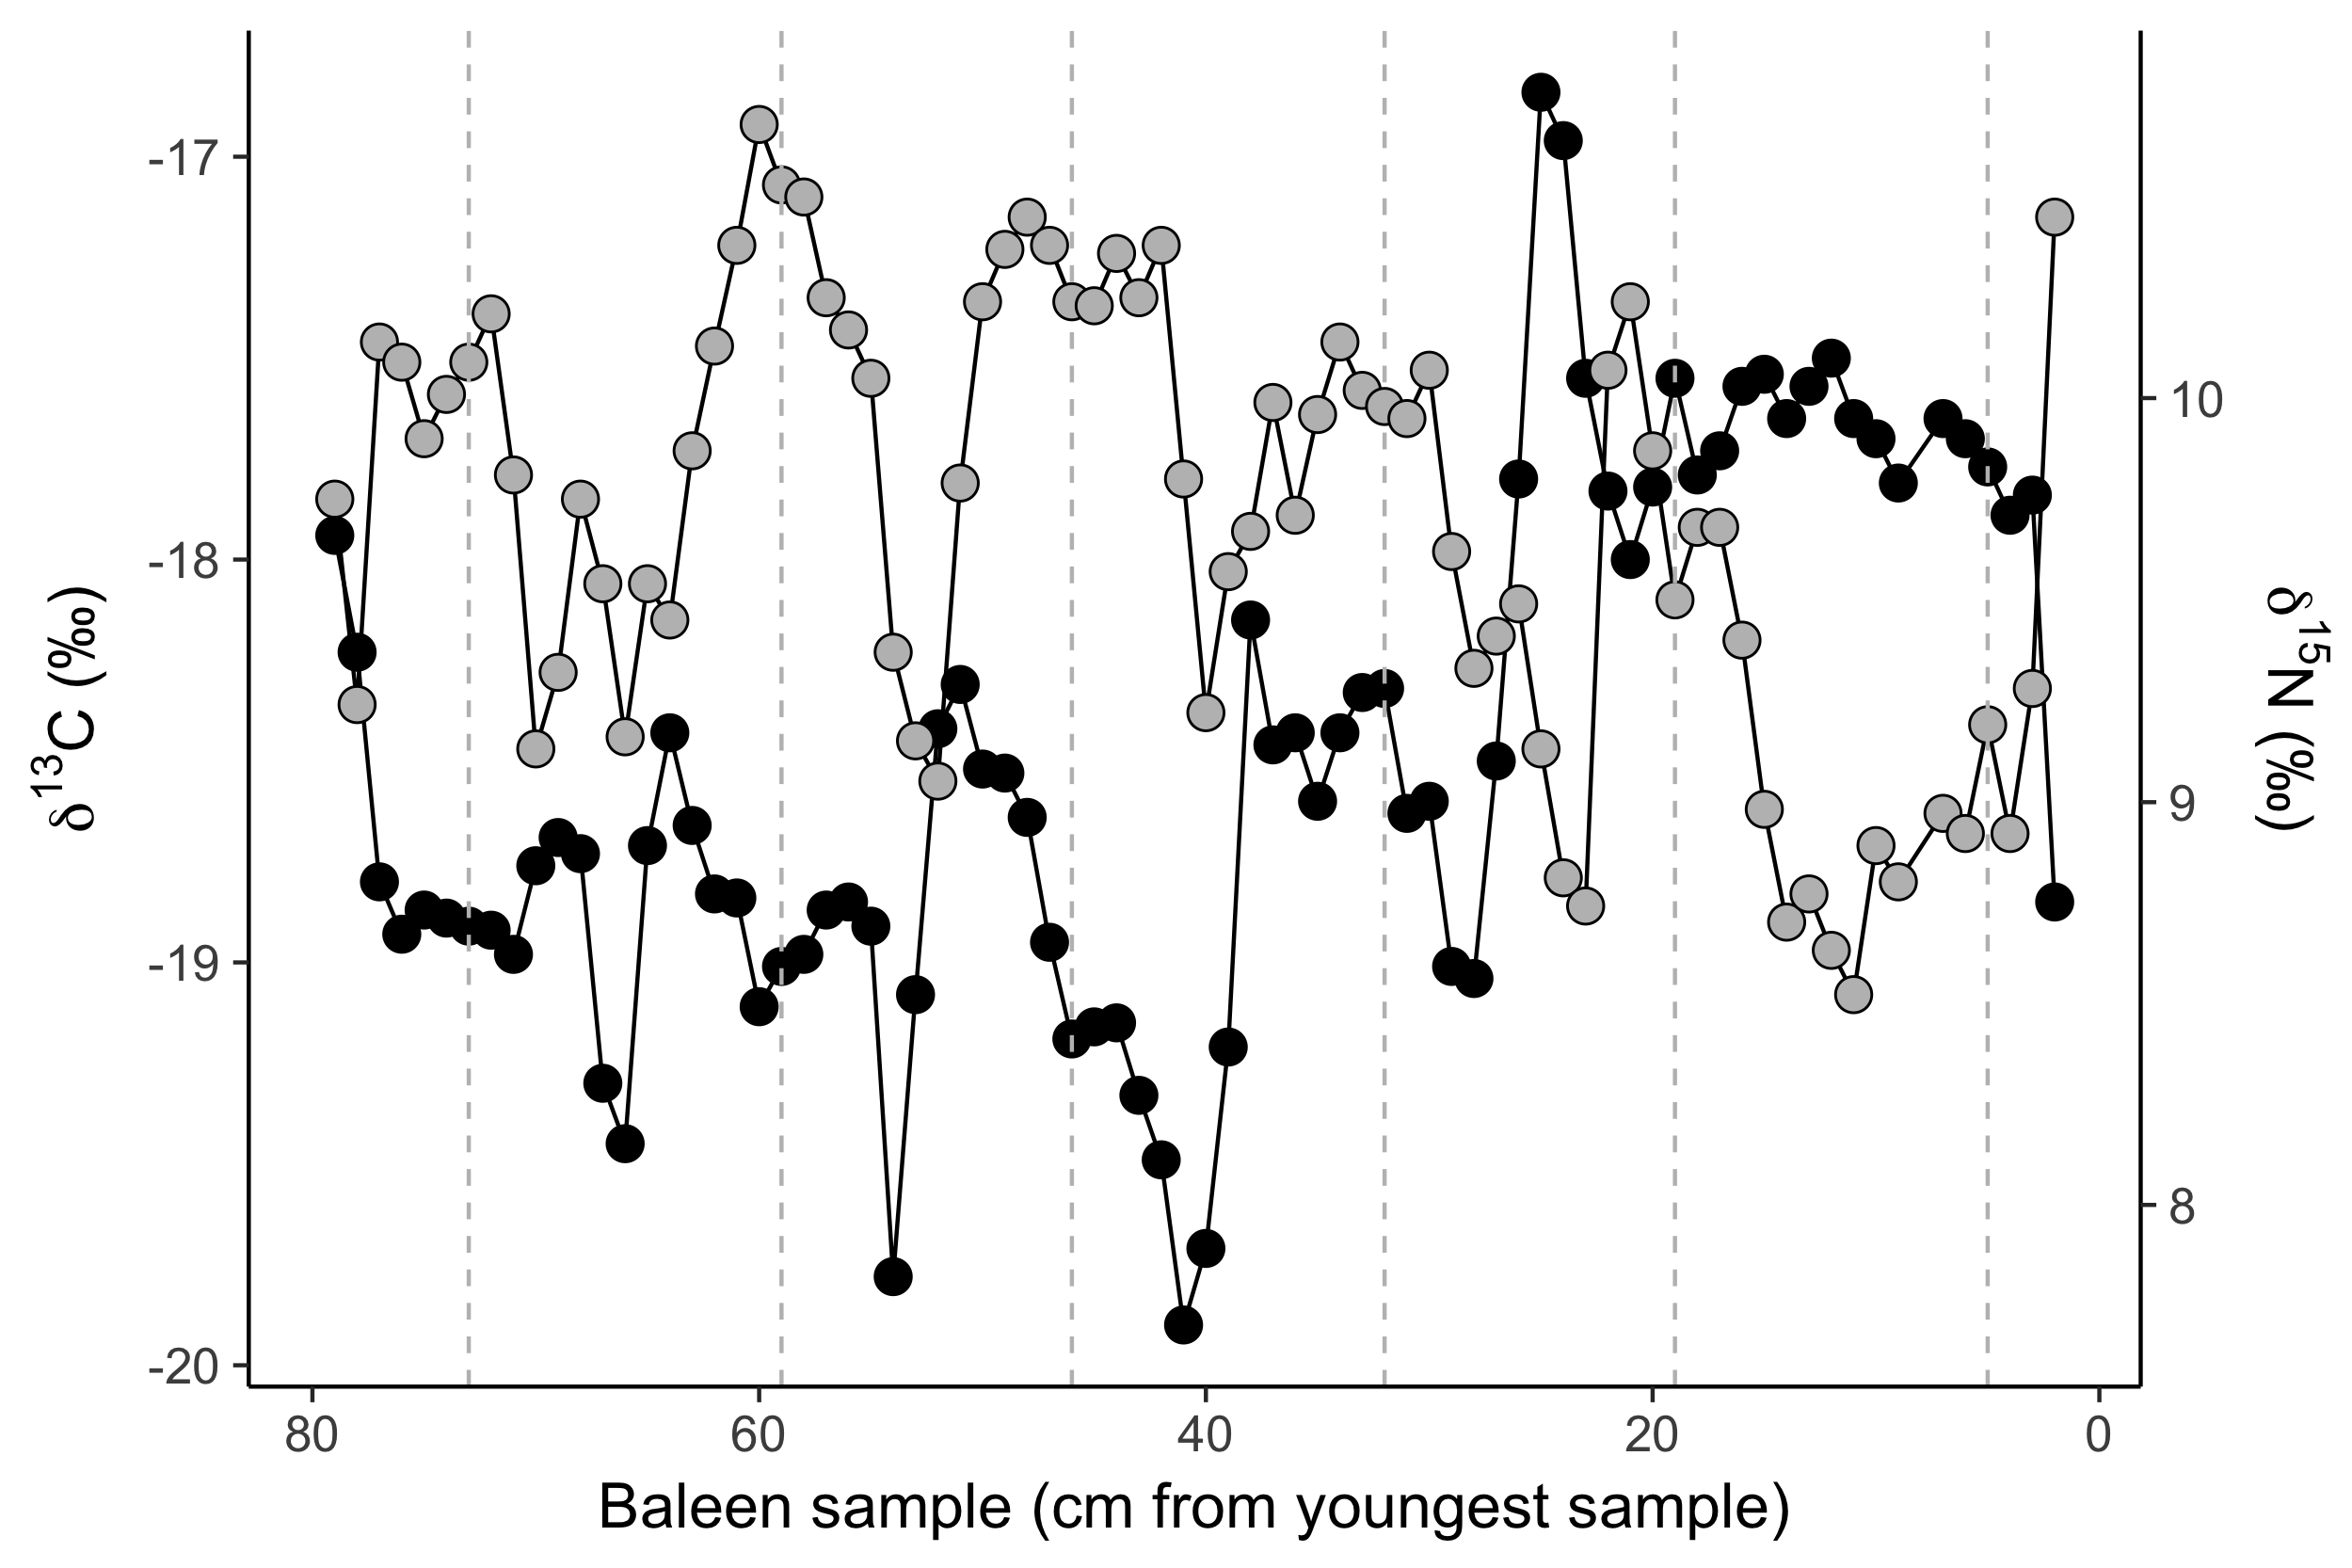
\includegraphics[width = \linewidth]{figures/Figure-1a-raw-dC-dN-data.png}
  \label{fig11a}
  \caption{One panel figure}
\end{figure}

% one panel of the real trace
\begin{figure}
  \centering
  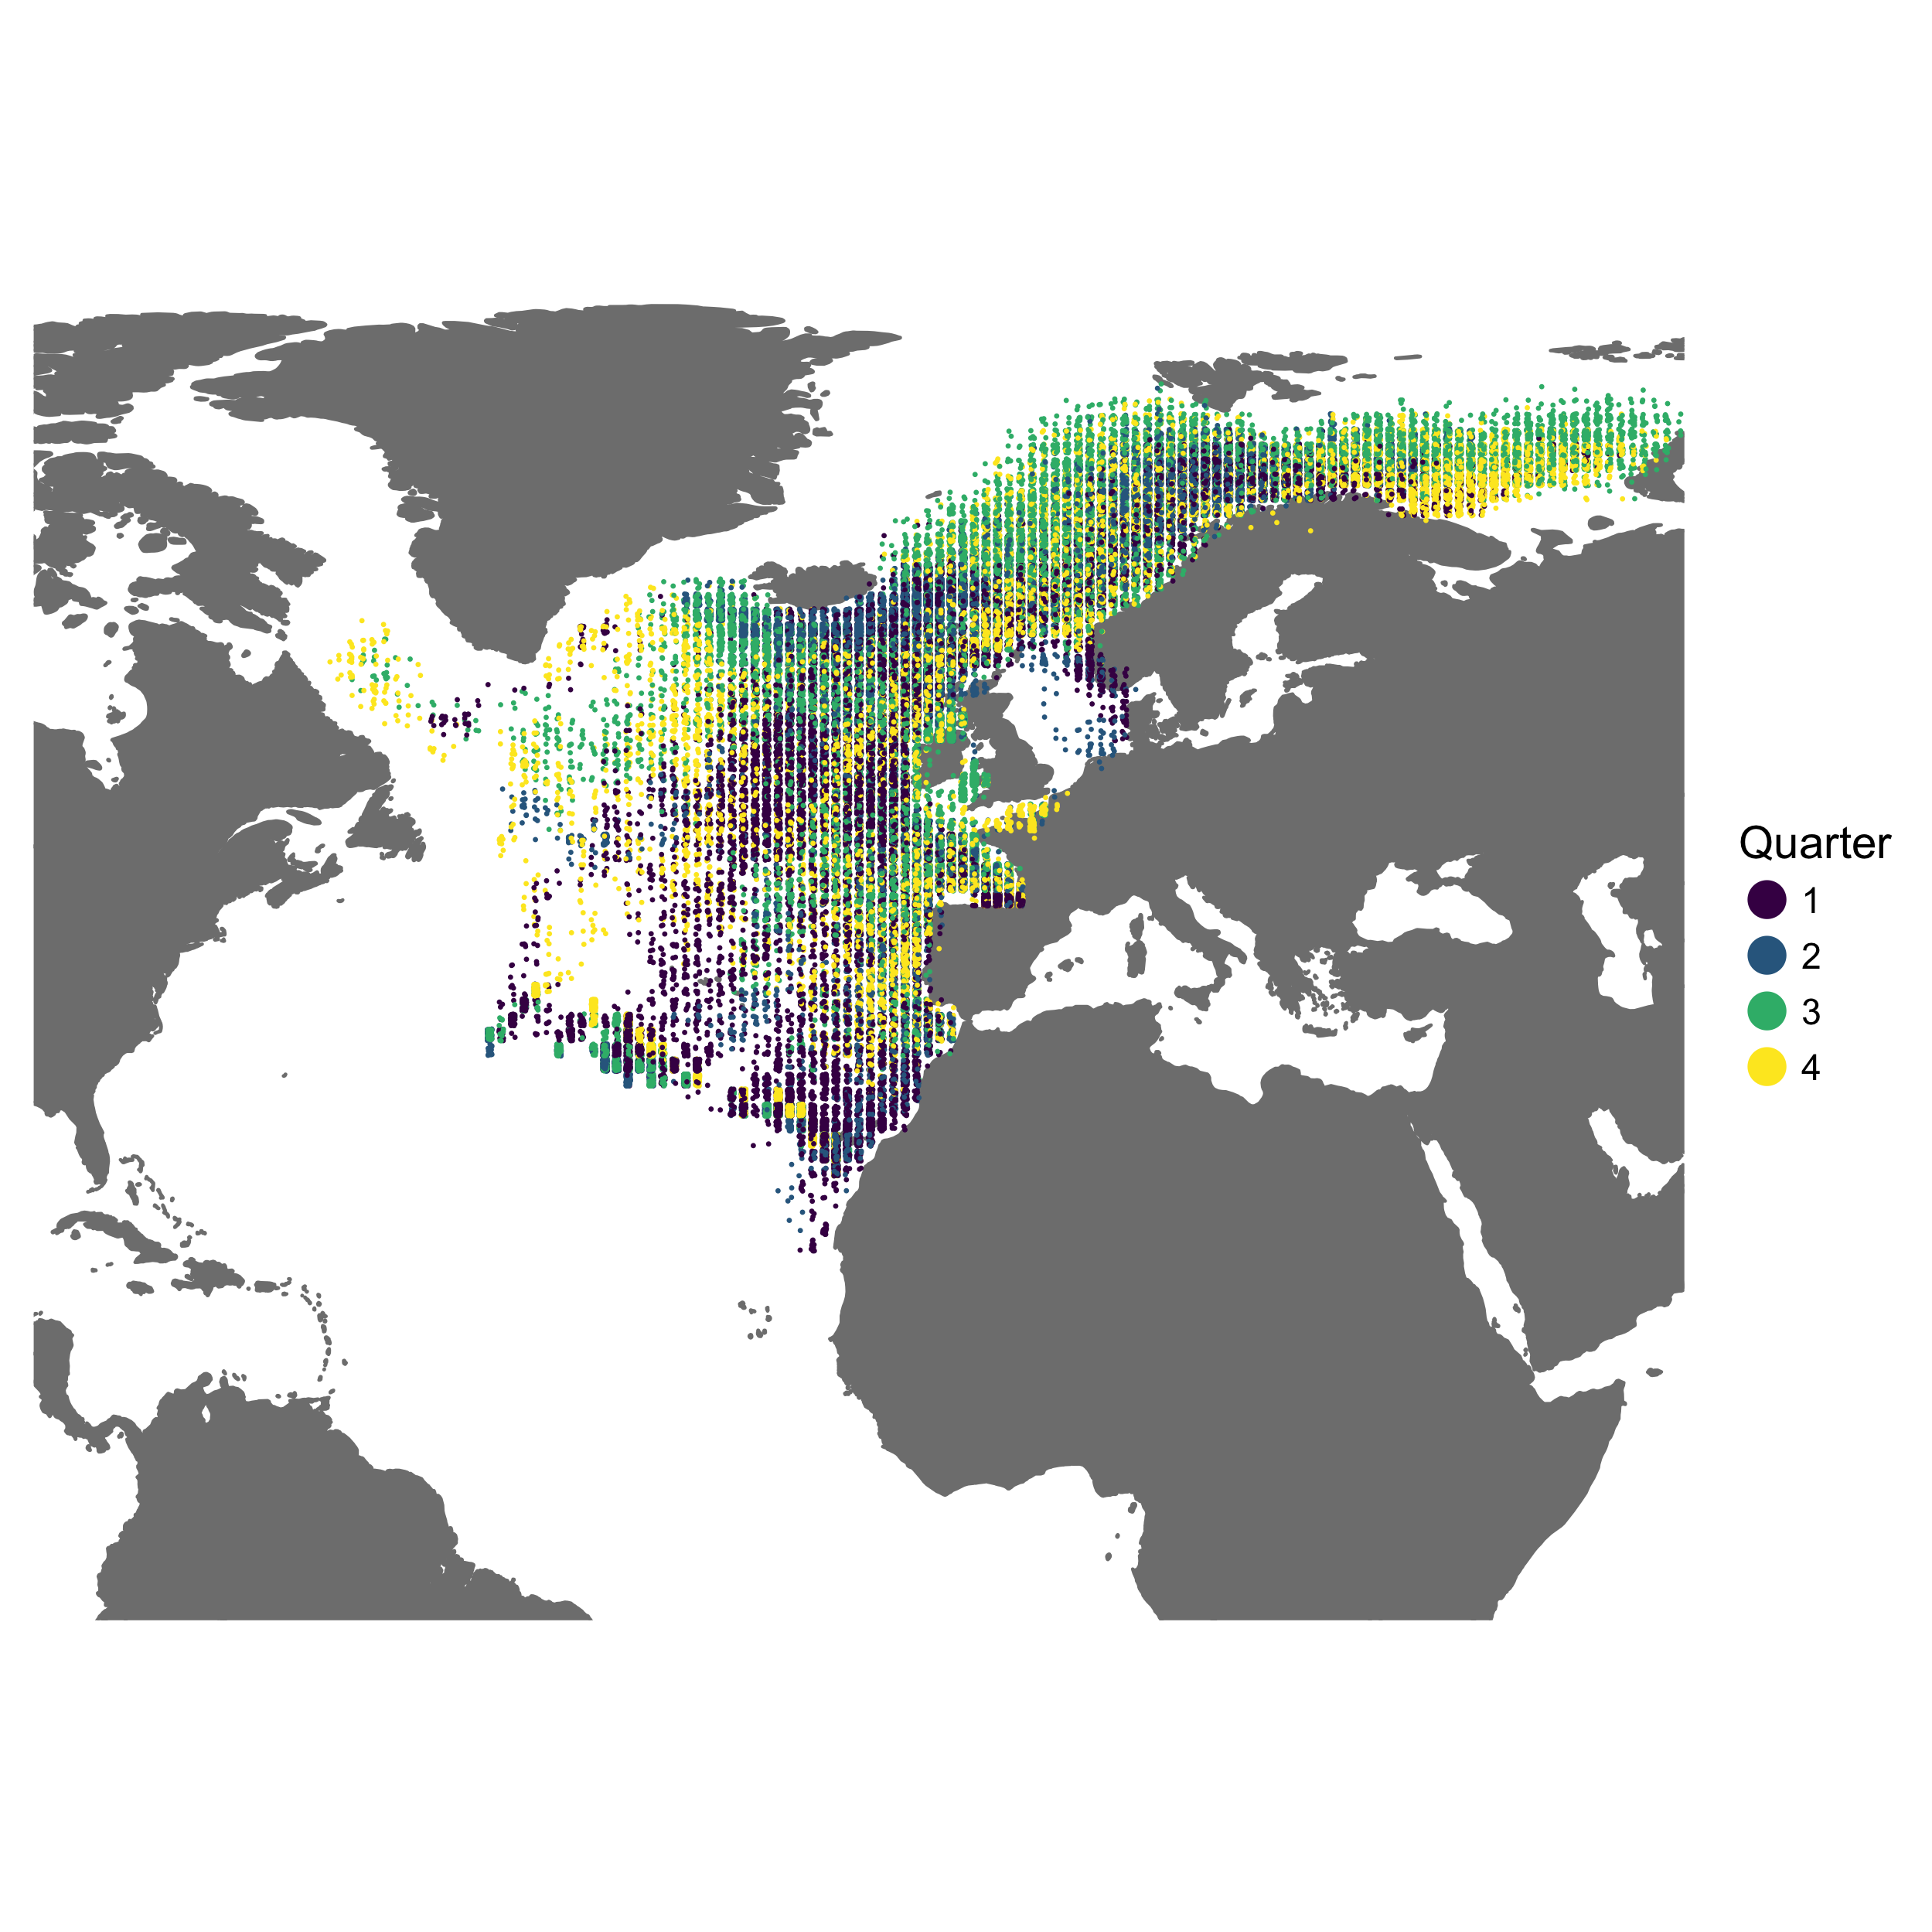
\includegraphics[width = \linewidth]{figures/Figure-1b-migratory-model-full-map.png}
  \label{fig11b}
  \caption{One panel figure}
\end{figure}

% one panel of the real trace
\begin{figure}
  \centering
  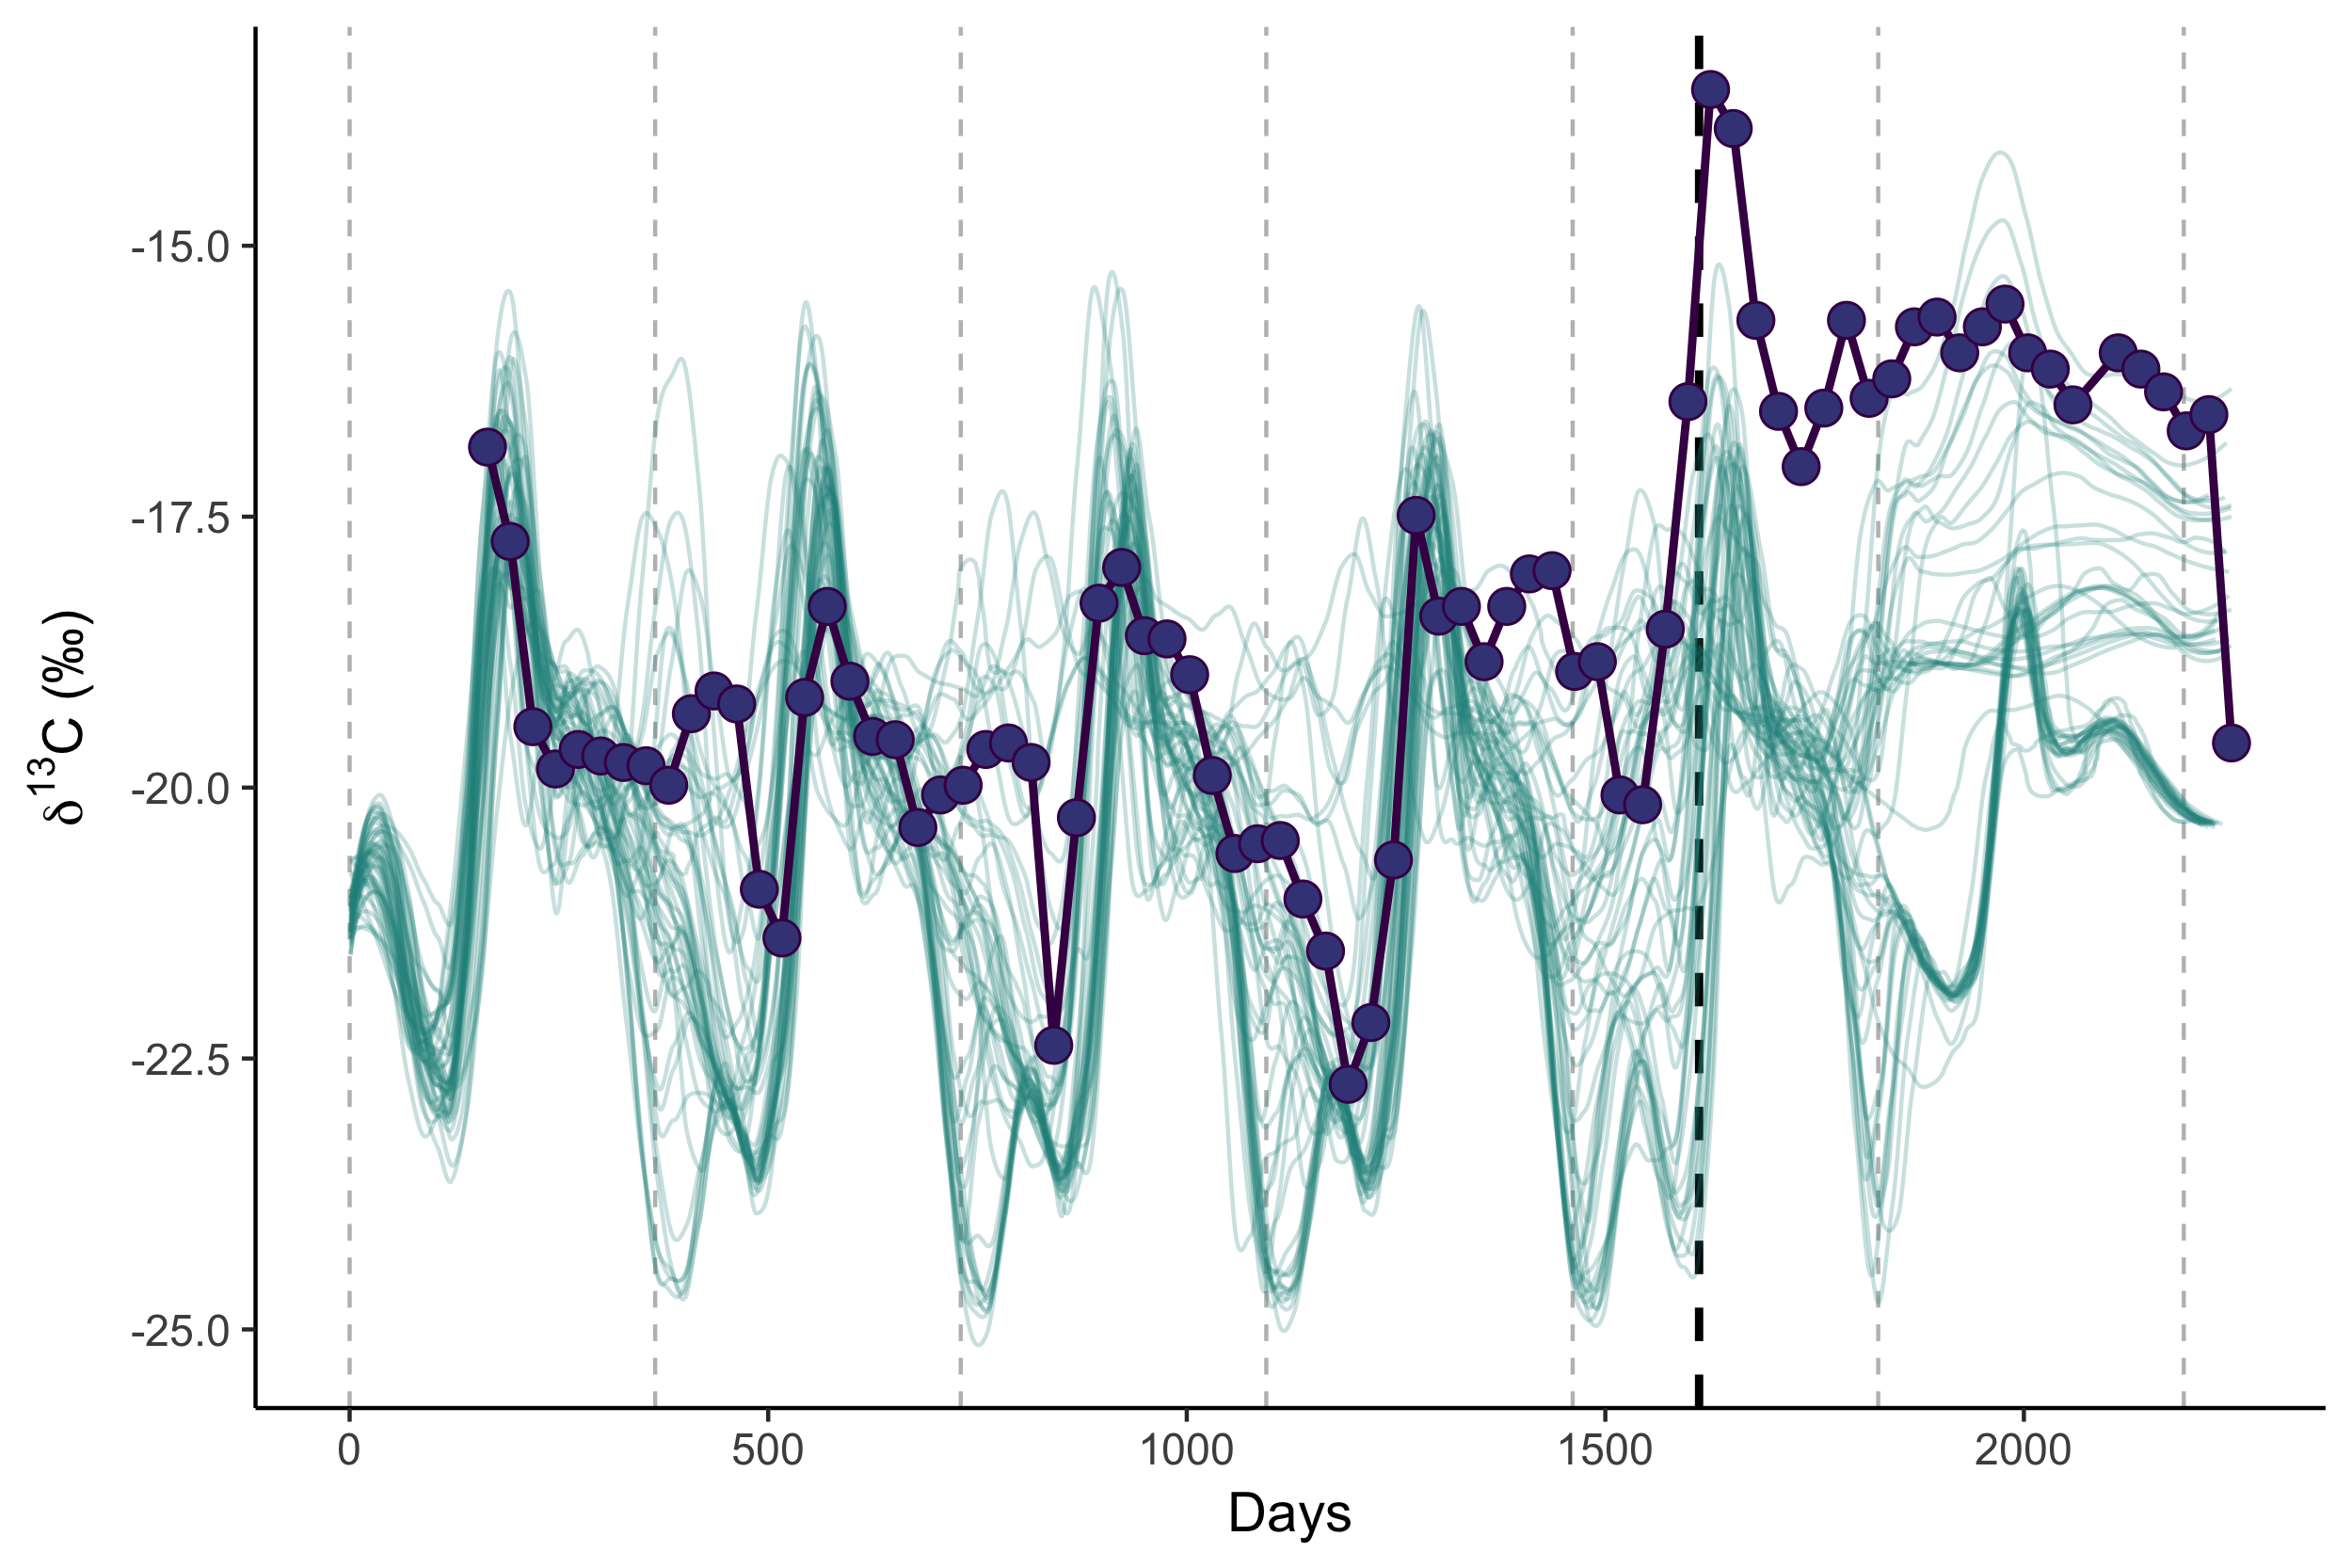
\includegraphics[width = \linewidth]{figures/Figure-1c-migratory-model-d13C.png}
  \label{fig11c}
  \caption{One panel figure}
\end{figure}

 
To interpret these isotopic signatures, we simulated time series of $\delta^{13}$C and $\delta^{15}$N values expected under differing movement behaviours, by coupling a novel agent-based model of whale movements (see Supplementary Methods) to models of global phytoplankton $\delta^{13}$C and $\delta^{15}$N values\cite{magozzi2017using} (Schmittner and Somes). 
We simulated the movement of the whale with the likelihood, direction, and extent of movement influenced by behavioural state, sea surface temperature, water depth and phytoplankton concentration (as a proxy for zooplankton food availability). 
At each time point and location in the simulations, we extracted phytoplankton $\delta^{13}$C and $\delta^{15}$N values from the models\cite{magozzi2017using} (Schmittner and Somes) resulting in a range of simulated isotopic profiles for different migration patterns and foraging areas. 
We then determined which of these simulated profiles were biogeochemically consistent with the isotopic profile of the blue whale's baleen (Fig. 1) and use this to interpret the results.
 
During behavioural phase one, the whale is foraging at high northern latitudes, likely off the coast of Norway. 
The pronounced cyclical variations in $\delta^{13}$C values are characteristic of the isotopic expression of the spring phytoplankton bloom in northern waters\cite{magozzi2017using}. 
This interpretation is also consistent with the relatively negative median $\delta^{13}$C values (Fig. 1). 
The periodicity of $\delta^{13}$C and $\delta^{15}$N values is explained by short distance seasonal migrations, with the whale overwintering off the coast of Ireland. 
The relatively positive and invariant $\delta^{13}$C values seen during behavioural phase two are found in subtropical areas, particularly off the coast of the Azores, suggesting the whale migrated rapidly to southerly latitudes in early 1889, but continued feeding (other mysticete whales fast during migrations, but blue whales are too large to stop feeding for long periods\cite{busquets2017estimating}?silva paper). 
The whale remained in these warm waters for over a year and was returning to her northern feeding grounds when she became stranded. 
 
Movement to warm waters alone, however, cannot explain the dramatic increase in $\delta^{13}$C values at the start of behavioural phase two. 
We believe that this reflects the physiological demands of pregnancy, as similar increases in $\delta^{13}$C values have been seen in pregnant South American sea lions\cite{cardona2017temporal}. 
The gradual increase in $\delta^{15}$N values to the autumn of 1890 is consistent with the isotopic expression associated with lactation\cite{cardona2017temporal}. Blue whales have a 10-12 month gestation period, and calves are weaned after 6-7 months\cite{handbook}. 
The proposed timescale of pregnancy around early spring 1889, birth in spring 1890, lactation through summer 1890 and return to northern feeding grounds in early 1891 is therefore fully consistent with the known reproductive ecology of blue whales. 
This is the first quantitative evidence of historical movement patterns in blue whales, and reveals a fascinating snapshot into the life of an iconic specimen, where we previously only knew the date and location of its death. 
 
Conventional wisdom suggests that baleen whales migrate each year from feeding grounds near the poles in summer, to overwintering and breeding grounds nearer the equator\cite{corkeron1999baleen,lockyer1981migration}. 
However, a growing body of evidence suggests that not all whales migrate to subtropical waters each year, with some remaining at high latitudes year round\cite{mcdonald2006biogeographic}. 
Our results support this conclusion. 
Interestingly, there is still a resident population of blue whales in the region our models place the blue whale within, and females still breed in the subtropical waters near the Azores\cite{reilly2008balaenoptera}. 
This suggests that whale movements have remained similar over hundreds of years, despite changes in anthropogenic pressures. 
Whaling was an intense pressure for blue whales during the period we are analysing. 
Before whaling in the North Atlantic began in 1868\cite{reilly2008balaenoptera}, there were 10,000-15,000 blue whales in the region\cite{sigurjonsson1995life}. 
By 1900 fisheries had moved outside the area because stocks were so depleted\cite{reilly2008balaenoptera}; during this period over 12,000 blue whales were landed\cite{sigurjonsson1995life}. 
The NHM blue whale thus represents an individual from a species at the brink of extinction. 
Blue whales were the first species that humans legislated to save, and represent a big conservation success story, although North Atlantic stocks have not recovered to the same extent as other whales in the region\cite{sigurjonsson1995life,pike2009note}. 
There is also evidence that blue whales are shifting their ranges due to warming waters off Iceland\cite{10.3389/fevo.2015.00006}. 
Thus understanding historical movements of North Atlantic blue whales has never been more vital if we wish to preserve them for future generations.
 
In conclusion, the model we present here allows us to recreate individual-level movement behaviours and life history using tissues from museum collections and other sources. 
This has applications beyond this individual whale, and beyond cetaceans, as our model can be applied to any marine species with constantly growing tissues, for example seal whiskers, shark skin, and fish scales. 
These techniques can also allow us study extinct species' behaviours and understand how populations were affected by past pressures such as hunting, and present-day pressures such as global change. 
Finally, our results highlight that museums represent a vast, mostly untapped, treasure trove of information ready for us to explore.


\section{Methods (condensed)}
%<3000 words
% no figures no tables

\subsection{Stable isotope extractions from baleen}
Baleen was collected from the Natural History Museum, London (specimen BMNH.1892.3.1.1). 
The baleen plate was cleaned with ethanol to remove surface contaminants. 
{\raise.17ex\hbox{$\scriptstyle\sim$}}1mg samples of keratin powder were then collected from the plate using a hand-held drill and grinding bit. 
78 samples were taken at 1cm intervals, 0.5cm from the outer edge of the plate, starting at the proximal section which contains the most recent tissue. 
Baleen grows at a constant rate, so the samples are equally spaced through time\cite{best1996stable}. Carbon and nitrogen isotope analysis was performed simultaneously via continuous-flow isotope ratio mass spectrometry at the National Oceanographic Centre (Southampton, UK), using a Vario Isotope select elemental analyser, coupled with Isoprime 100 isotope mass spectrometer. 
Replicates using internal laboratory standards (L-glutamic acid (C), Glutamic acid (CT standard), acetanilide and protein standard OAS) were used for quality control and calibration. 
C:N ratios for samples ranged from 3.28\text{\textperthousand} to 3.72\text{\textperthousand}, well within the acceptable theoretical range for pure keratin ($3.4\pm0.5$) allowing for comparison among samples (Hobson  Koch 1998). 
 
\subsection{Time calibrating stable isotope profiles}
Seasonal migrations across isotopic gradients induce cyclical variations in the isotopic composition of baleen, the distance between cycles reflecting growth rates\cite{hobson1998stable,busquets2017estimating}. 
Clear periodicity was evident in $\delta^{15}$N values across the entire baleen plate, and in $\delta^{13}$C values in the most distal (oldest) 65cm of the plate. 
We calculated isotopic periodicity within the baleen sample using Fourier Transform analysis\cite{cardona2017temporal}, revealing a consistent growth rate of 13.5cm $y^{-1}$ which is remarkably similar to the mean isotope-derived baleen growth rates of $15.5 \pm 2.2cm y{^-1}$ estimated for six blue whales from the Californian Pacific\cite{busquets2017estimating}.  
Therefore we dated the youngest baleen sample as 1st March 1891, 24 days prior to the stranding date, 25th March 1891. 
Cross-correlation analysis (ref?) demonstrated a strong negative covariance between $\delta^{13}$C and $\delta^{15}$N values within behavioural phase one (oldest 60cm of the baleen plate), but no relationship between $\delta^{13}$C and $\delta^{15}$N values during behavioural phase two.
 
\subsection{Baseline isotope comparisons}
Isotope-enabled biogeochemical ocean models\cite{magozzi2017using} (Schmittner and Somes) were used to characterize the isotopic composition of phytoplankton expected in different potential foraging grounds. 
Annual average $\delta^{15}$N POM (particulate organic matter) values were provided by Somes (pers.comm) based on a 5$^{\circ}$ resolution biogeochemical model. 
$\delta^{13}$C POM values were simulated at 1$^{\circ}$ and monthly resolution using an isotopic extension to the NEMO-MEDUSA ocean biogeochemical model\cite{magozzi2017using,yool2013medusa}. 
Simulated  $\delta^{15}$N POM values are relatively positive in the northeast Atlantic north of c. 60$^{\circ}$N, and relatively negative in the central and southern North Atlantic. 
Annual average $\delta^{13}$C POM values largely vary with latitude, with more negative values in more northerly regions. 
In the central North Atlantic, $\delta^{13}$C POM values are relatively positive in the west, reflecting warm gulf stream waters (Fig S3). 
The isotopic composition of carbon in phytoplankton also varies through seasons as isotopic fractionation of carbon during photosynthesis is strongly influenced by sea surface temperature (Laws, Magozzi et al 2017). 
Thus temporal variations in $\delta^{13}$C POM values were superimposed on latitudinal gradients. 
The scale and nature of temporal variation in $\delta^{13}$C POM values also varies with latitude, with higher latitude seas showing greater intra-annual variation in $\delta^{13}$C POM values linked to strongly seasonal phytoplankton growth dynamics. 
We therefore used monthly simulated $\delta^{13}$C POM values to simulate the isotopic expression of phytoplankton expected to be encountered by whales exhibiting differing movement behaviours.
 
\subsection{Agent-based whale movement model}
Movement was coded as set of probabilistic rules. 
The parameters for these were taken from the literature on blue whale behaviour (e.g.\cite{handbook}). 
All terms were expressed as probability distributions allowing us to introduce individual variability. 
 
In the models, the likelihood of movement, direction (north, south, east, west, northeast, northwest, southeast, or southwest) and extent (1$^{\circ}$ or 2$^{\circ}$) of movement are all influenced by the following. 
(i) Behavioural state (migrating north, migrating south, foraging, or nursing). 
Northerly migrations were possible only in spring, and southerly migrations in autumn. Foraging was possible at anytime of year, and was triggered when whales encountered high concentrations of plankton. Nursing occurred at temperatures between 18 and 25$^{\circ}$C only. 
(ii) Sea surface temperature ($^{\circ}$C\cite{yool2013medusa}). 
When migrating north, whales were more likely to move towards lower temperatures provided they were above the minimum temperature threshold (3$^{\circ}$C); whereas whales migrating south sought warmer waters. 
(iii) Water depth (m; what reference is this collected from?). 
Whales were less likely to move into waters less than 400m deep, and increasingly unlikely to move into even shallower waters. 
(iv) Phytoplankton concentration (mmol N $m^{-3}$, for combined diatom and non-diatom communities\cite{yool2013medusa}). 
This was included as a proxy for zooplankton food availability. 
Whales are more likely to move towards (or remain within) areas of high phytoplankton density, particularly during the foraging behavioural state. 
 
We simulated the isotopic expression expected for (a) residency in each known hotspot for blue whale sightings or historic hunting grounds in the North Atlantic (Norwegian/Barents Sea, West Ireland, South Greenland, Nova Scotia/Newfoundland and Canaries/Azores\cite{mcdonald2006biogeographic,reilly2008balaenoptera,sigurjonsson1995life}; Fig SX; (b) seasonal migration between high sub-arctic latitudes and temperate latitudes around the British Isles and (c) seasonal migration between high latitudes and subtropical latitudes. 
Various movement rules were implemented to avoid simulations ending up on land, or becoming `stuck' in the relatively shallow waters of the Bay of Biscay or the Strait of Dover. 
For a full description of the model and its parameters see Supplementary Methods. 
We simulated whale movements XX times for each scenario and residency hotspot. 
For each movement simulation we extracted phytoplankton $\delta^{13}$C and $\delta^{15}$N values at each time point and location from the models described above\cite{magozzi2017using} (Somes). 
We then compared the simulated stable isotope profiles (Fig. S4) to the profile of the blue whale (Fig. 1).
 
\subsection{Data Availability}
Data are available on the Natural History Museum, London's data portal (https://data.nhm.ac.uk). 
R code is available from XXX.

% References

\bibliographystyle{nature}
\bibliography{blue-whale}

\section{Supplementary Information}
Supplementary Information is linked to the online version of the paper at www.nature.com/nature.

\section{Acknowledgments}
% adjectives not allowed!
This work was funded by the British Ecological Society (grant: 5771/6815). 
We thank XXX for comments on drafts.
We thank CJ Somes for providing  $\delta^{15}$N POM data.

\section{Author contributions}
% rough draft at present feel free to edit
CT, NC, AJ, RS, and KC collected baleen from the NHM collections. 
KC and CT extracted and analysed samples.
CT created the movement model.
EC, NC and RS helped parameterise the model.
AJ created the figures. 
NC, CT and EC wrote the paper.
All authors edited drafts and approved the final version.

\section{Author information}
Reprints and permissions information is available at www.nature.com/reprints.
The authors declare no competing financial interests.
Correspondence and requests for materials should be addressed to natalie.cooper@nhm.ac.uk.
% One person only allowed

%\section{Tables}

%\section{Figure legends}


%\newpage
%\section{Figures}

%  \begin{figure}[!htbp]
%    \centering
%      \includegraphics[width=12cm]{XXX.pdf}
%      \caption{}
%      \label{}
%  \end{figure}

\end{document}